\documentclass[18pt, letterpaper]{article}
\usepackage[left=2.5cm, right=2.5cm]{geometry}
\usepackage{soul}
\usepackage[T1]{fontenc}
\usepackage{hyperref}
\usepackage{graphicx}
\usepackage{gensymb}
\usepackage{float}
\title{Analiza zależności zanieczyszczenia powietrza od cykli czasowych i pogody}
\author{Michał Włodarczyk \\ Politechnika Wrocławska \\ Informatyka Stosowana \\ MSiD Lab Śr 15:15 P \\ }
\date{8 Czerwca 2024}
\begin{document}



\begin{titlepage}
\maketitle
\vspace{10em}
\tableofcontents
\end{titlepage}



\section{Wstęp}

 Tematem poniższej analizy są zależności między zanieczyszczeniem powietrza w dużym mieście a czasem (pora dnia, pora roku, dzień tygodnia) i warunkami pogodowymi, na przykładzie Wrocławia. Celem jest wyszczególnienie istotnych zależności, w miarę możliwości podanie ich potencjalnych przyczyn, oraz podjęcie próby stworzenia modelu przewidującego wartości przyjętych metryk na podstawie informacji czasowej i danych pogodowych.




 
\section{Zbiór danych}

Użyty zbiór danych składa się z dwóch głównych komponentów: dane dotyczące zanieczyszczenia powietrza, pozyskane z publicznych zbiorów Głównego Inspektoratu Ochrony Środowiska\cite{pollution_source}, oraz dane pogodowe pozyskane z publicznych zbiorów Instytutu Meteorologii i Gospodarki Wodnej\cite{weather_source}. Dane w obu zbiorach są rejestrowane co godzinę (z obu źródeł można również uzyskać dane dzienne, ale jako że nie zawierają one żadnych użytecznych informacji nie zawartych w danych godzinowych nie zostały one uwzględnione w analizie).

\subsection{Dane dotyczące zanieczyszczenia powietrza}

Dane dotyczące zanieczyszczeń powietrza są dostępne z lat 2000-2022 z wielu stacji pomiarowych, w tym kilku na terenie Wrocławia. Niestety, dane z wielu lat, zwłaszcza przed rokiem 2015, są fragmentaryczne, z niekiedy kilkumiesięcznymi przerwami w raportowaniu. Ponadto nie wszystkie stacje pomiarowe zbierają dane dotyczące wszystkich wybranych do analizy metryk, również wiele stacji zostało zamkniętych lub otwartych w okresie 2000-2022 i dostępne są z nich dane tylko z części tego okresu. Ponieważ poszczególne stacje mogą istotnie się różnić zgłaszanymi pomiarami ze względu na swoje położenie, zrezygnowałem z łączenia danych z wielu stacji i ograniczyłem się do tych pochodzących ze stacji DsWrocWybCon (wybrzeże J. Conrada-Korzeniowskiego 18), jako że są one stosunkowo kompletne. Dla każdej metryki z osobna odrzuciłem dane z lat z wieloma brakującymi wartościami (powyżej 5\%). W praktyce oznaczało to odrzucenie całości danych sprzed 2013 roku; stosunkowo pełne dane dla wszystkich metryk dostępne są dopiero od roku 2017. Brakujące wartości wypełniono przez interpolację; metoda ta sprawdza się dla niewielkiej liczby równomiernie rozłożonych brakujących wartości, ale doprowadziła by do znacznych zniekształceń gdyby zastosować ją do długich przerw które często zdarzają się w latach przed 2015.

Kierując się m. in. informacjami ze strony internetowej Programu Środowiskowego ONZ \cite{un_air_pollution} wybrałem sześć metryk reprezentujących stopień zanieczyszczenia powietrza. Są to stężenia następujących substancji: 
\begin{itemize}
\item tlenek węgla (CO)
\item dwutlenek azotu (NO2)
\item ozon troposferyczny (O3)
\item dwutlenek siarki (SO2)
\item pył zawieszony o średnicy nie większej niż 2.5 mikrometra (PM25)
\item pył zawieszony o średnicy nie większej niż 10 mikrometrów (PM10)
\end{itemize}
Stężenie tlenku węgla jest podawane w miligramach na metr sześcienny, stężenia pozostałych substancji w mikrogramach na metr sześcienny.

\subsection{Dane pogodowe}
Dane pogodowe są na szczęście o wiele wyższej jakości: praktycznie nie ma brakujących wartości i dostępne są dane dotyczące całego interesującego nas okresu z jednej stacji meteorologicznej (Wrocław-Strachowice). 

Z danych pogodowych wyodrębniłem do analizy sześć zmiennych: 
\begin{itemize}
\item kierunek wiatru [\degree] (do większości zastosowań został zamieniony na zmienną kategoryczną)
\item prędkość wiatru [m/s]
\item temperatura [\degree C]
\item wilgotność [\%]
\item ciśnienie atmosferycze [hPa]
\item wielkość opadów [mm]
\end{itemize}
Istotną cechą zbioru jest to, że pomiary wielkości opadów są raportowane co 6 godzin (w godzinach (0:00, 6:00, 12:00,18:00), a w pozostałych rekordach wielkość opadów zawsze wynosi zero. W niektórych wizualizacjach i eksperymentach wymusza to dodatkowe operacje na danych, np. ich uśrednianie za pomocą okna przesuwnego o długości 6 lub pomijanie rekordów z pozostałych godzin.



\section{Wstępne przetwarzanie danych}
\subsection{Dane dotyczące zanieczyszczenia powietrza}
Dane dotyczące zanieczyszczeń powietrza wymagały znacznego przetworzenia z powodu niejednolitego formatu i dużej ilości brakujących danych. W pierwszym kroku dane wczytano z plików .xslx (przy czym pojedynczy plik zawierał wartości jednej metryki w danym roku dla różnych stacji pomiarów), nadano im jednolity format (wymagało to m. in. usunięcia niepotrzebnych wierszy nagłówkowych, ustawienia kropki jako separatora dziesiętnego w plikach w których zamiast niej użyto przecinka, zaktualizowania starych kodów stacji pomiarowych i zaokrąglenia czasów do pełnych godzin w celu pozbycia się niewielkich niedokładności czasowych) i wyekstraktowano kolumny odpowiadające stacjom pomiarowym na terenie Wrocławia. W drugim kroku dokonano analizy ilości brakujących danych w poszczególnych plikach i na jej podstawie dokonano selekcji danych do dalszej analizy, wybierając nieprzerwane ciągi lat w których odsetek brakujących wartości przekraczał 5\%, po czym w tak wyselekcjonowanych danych uzupełniono brakujące wartości. 
\subsection{Dane pogodowe}
Dane pogodowe w porównaniu niemal nie wymagały wstępnego przetwarzania. Jedyne czynności jakie wykonano przed rozpoczęciem analizy to scalenie w jedną kilku kolumn przechowujących informacje czasową oraz wyekstraktowanie z dużej liczby zmiennych wybranych sześciu.


\section{Analiza eksploracyjna}

\subsection{Rozkład danych}

W ramach analizy eksploracyjnej wygenerowano wizualizacje rozkładów poszczególnych zmiennych i metryk.

\subsubsection{CO}
\begin{figure}[H]
\centering
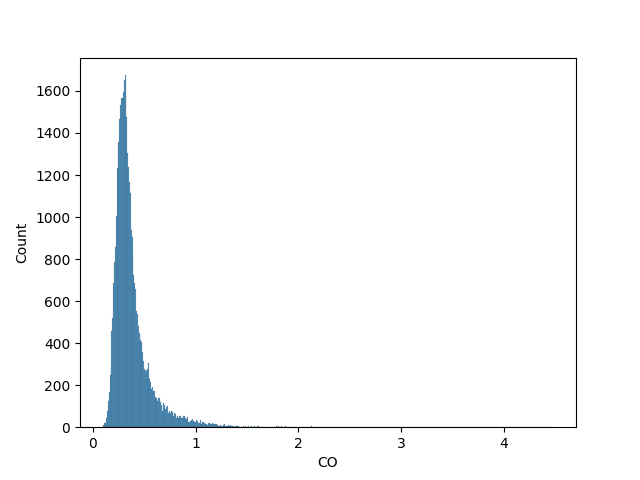
\includegraphics[width=120mm, height=90mm]{visualisations/histograms/CO_hist.png}
\caption{Histogram stężenia CO}
\end{figure}
\begin{table}[H]
\centering
\begin{tabular}{|c|c|c|c|}
\hline
Min.  & Max. & Średnia & Odchylenie \\ \hline
0.094 & 4.48 & 0.378   & 0.197      \\ \hline
\end{tabular}
\caption{Parametry opisujące rozkład stężenia CO}
\end{table}

\subsubsection{NO2}
\begin{figure}[H]
\centering
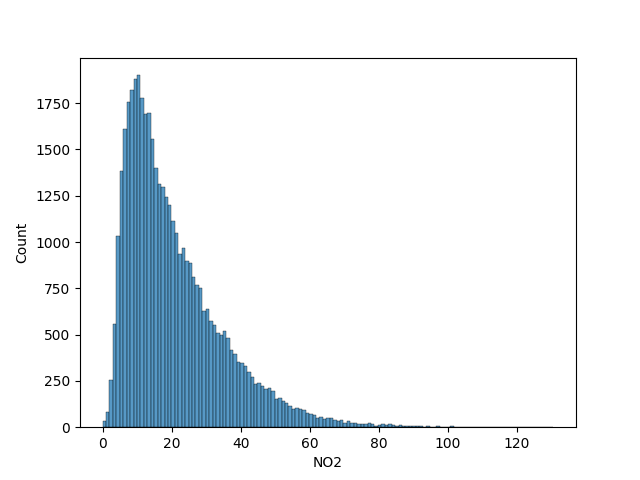
\includegraphics[width=120mm, height=90mm]{visualisations/histograms/NO2_hist.png}
\caption{Histogram stężenia NO2}
\end{figure}
\begin{table}[H]
\centering
\begin{tabular}{|c|c|c|c|}
\hline
Min.  & Max. & Średnia & Odchylenie \\ \hline
0 & 165.31 & 20.5   & 14.41      \\ \hline
\end{tabular}
\caption{Parametry opisujące rozkład stężenia NO2}
\end{table}

\subsubsection{O3}
\begin{figure}[H]
\centering
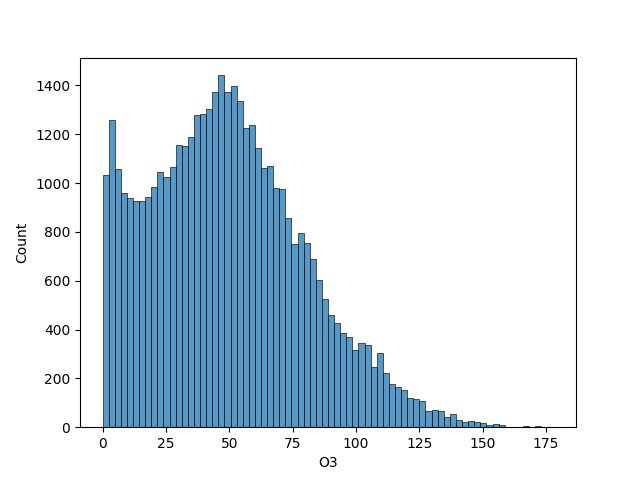
\includegraphics[width=120mm, height=90mm]{visualisations/histograms/O3_hist.png}
\caption{Histogram stężenia O3}
\end{figure}
\begin{table}[H]
\centering
\begin{tabular}{|c|c|c|c|}
\hline
Min.  & Max. & Średnia & Odchylenie \\ \hline
0 & 177.94 & 49.2   & 30.38      \\ \hline
\end{tabular}
\caption{Parametry opisujące rozkład stężenia O3}
\end{table}

\subsubsection{SO2}
\begin{figure}[H]
\centering
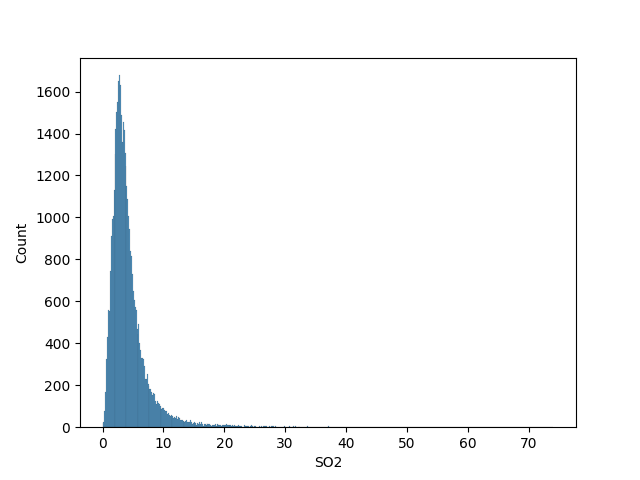
\includegraphics[width=120mm, height=90mm]{visualisations/histograms/SO2_hist.png}
\caption{Histogram stężenia SO2}
\end{figure}
\begin{table}[H]
\centering
\begin{tabular}{|c|c|c|c|}
\hline
Min.  & Max. & Średnia & Odchylenie \\ \hline
0 & 74.08 & 4.5   & 3.54      \\ \hline
\end{tabular}
\caption{Parametry opisujące rozkład stężenia SO2}
\end{table}

\subsubsection{PM25}
\begin{figure}[H]
\centering
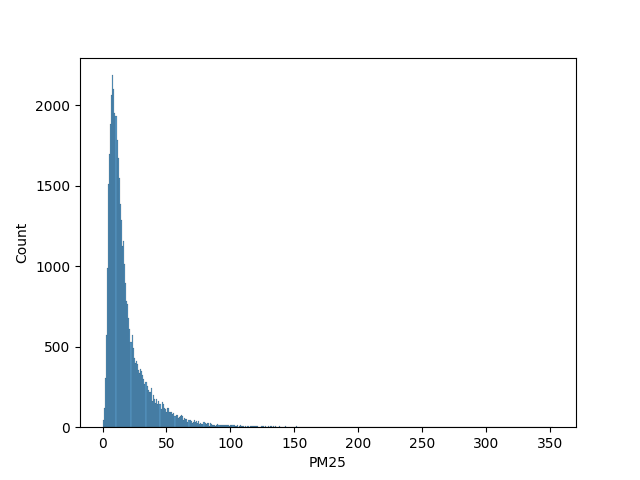
\includegraphics[width=120mm, height=90mm]{visualisations/histograms/PM25_hist.png}
\caption{Histogram stężenia PM25}
\end{figure}
\begin{table}[H]
\centering
\begin{tabular}{|c|c|c|c|}
\hline
Min.  & Max. & Średnia & Odchylenie \\ \hline
0 & 352.63 & 18.87   & 18.33      \\ \hline
\end{tabular}
\caption{Parametry opisujące rozkład stężenia PM25}
\end{table}

\subsubsection{PM10}
\begin{figure}[H]
\centering
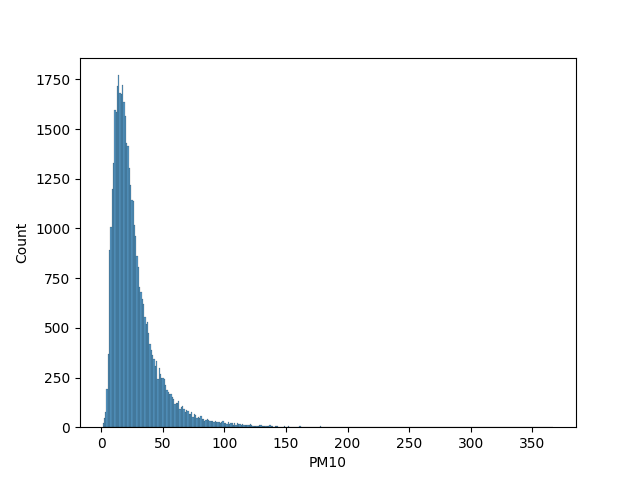
\includegraphics[width=120mm, height=90mm]{visualisations/histograms/PM10_hist.png}
\caption{Histogram stężenia PM10}
\end{figure}
\begin{table}[H]
\centering
\begin{tabular}{|c|c|c|c|}
\hline
Min.  & Max. & Średnia & Odchylenie \\ \hline
0.95 & 367.29 & 26.72   & 20.34      \\ \hline
\end{tabular}
\caption{Parametry opisujące rozkład stężenia PM10}
\end{table}

\subsubsection{Kierunek wiatru}
\begin{figure}[H]
\centering
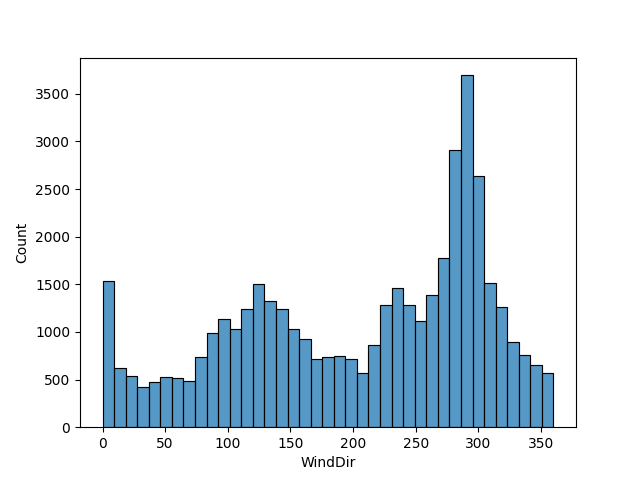
\includegraphics[width=120mm, height=90mm]{visualisations/histograms/WindDir_hist.png}
\caption{Histogram kierunku wiatru}
\end{figure}

\subsubsection{Prędkość wiatru}
\begin{figure}[H]
\centering
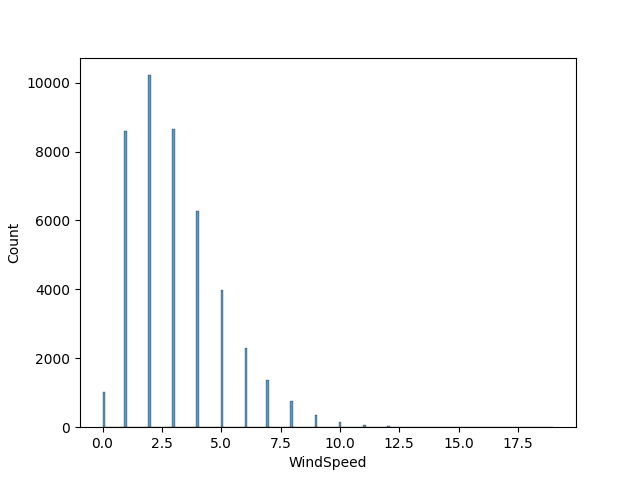
\includegraphics[width=120mm, height=90mm]{visualisations/histograms/WindSpeed_hist.png}
\caption{Histogram prędkość wiatru}
\end{figure}
\begin{table}[H]
\centering
\begin{tabular}{|c|c|c|c|}
\hline
Min.  & Max. & Średnia & Odchylenie \\ \hline
0 & 19 & 3.11   & 1.99      \\ \hline
\end{tabular}
\caption{Parametry opisujące rozkład prędkości wiatru}
\end{table}

\subsubsection{Temperatura}
\begin{figure}[H]
\centering
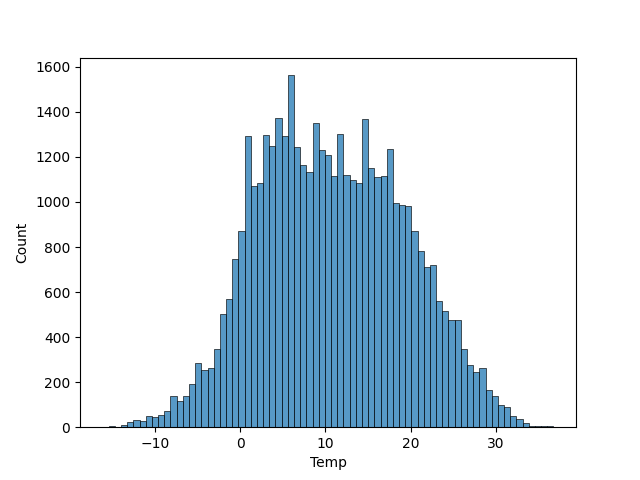
\includegraphics[width=120mm, height=90mm]{visualisations/histograms/Temp_hist.png}
\caption{Histogram temperatury}
\end{figure}
\begin{table}[H]
\centering
\begin{tabular}{|c|c|c|c|}
\hline
Min.  & Max. & Średnia & Odchylenie \\ \hline
-16.2 & 37.1 & 10.83   & 8.57      \\ \hline
\end{tabular}
\caption{Parametry opisujące rozkład temperatury}
\end{table}

\subsubsection{Wilgotność}
\begin{figure}[H]
\centering
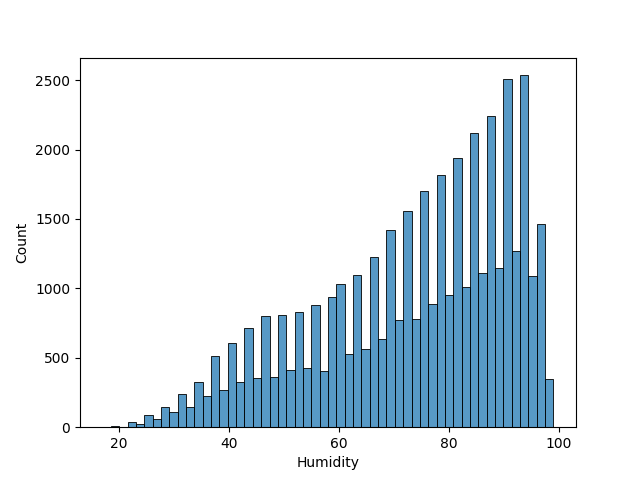
\includegraphics[width=120mm, height=90mm]{visualisations/histograms/Humidity_hist.png}
\caption{Histogram wilgotności}
\end{figure}
\begin{table}[H]
\centering
\begin{tabular}{|c|c|c|c|}
\hline
Min.  & Max. & Średnia & Odchylenie \\ \hline
14 & 100 & 72.12   & 18.09      \\ \hline
\end{tabular}
\caption{Parametry opisujące rozkład wilgotności}
\end{table}

\subsubsection{Ciśnienie atmosferyczne}
\begin{figure}[H]
\centering
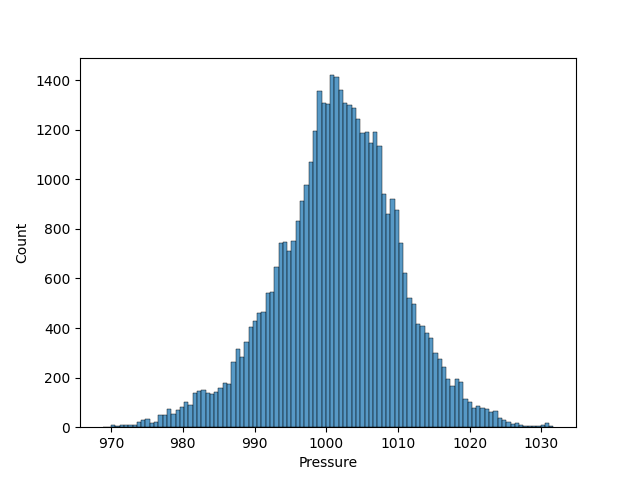
\includegraphics[width=120mm, height=90mm]{visualisations/histograms/Pressure_hist.png}
\caption{Histogram ciśnienia}
\end{figure}
\begin{table}[H]
\centering
\begin{tabular}{|c|c|c|c|}
\hline
Min.  & Max. & Średnia & Odchylenie \\ \hline
968.8 & 1031.7 & 1001.92   & 8.56      \\ \hline
\end{tabular}
\caption{Parametry opisujące rozkład ciśnienia}
\end{table}

\subsubsection{Wielkość opadów}
\begin{figure}[H]
\centering
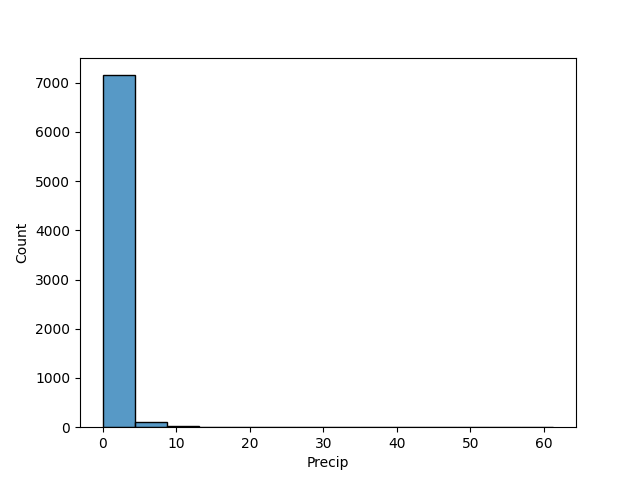
\includegraphics[width=120mm, height=90mm]{visualisations/histograms/Precip_hist.png}
\caption{Histogram wielkości opadów}
\end{figure}
\begin{table}[H]
\centering
\begin{tabular}{|c|c|c|c|}
\hline
Min.  & Max. & Średnia & Odchylenie \\ \hline
0 & 61.3 & 0.36   & 1.87      \\ \hline
\end{tabular}
\caption{Parametry opisujące rozkład wielkości opadów}
\end{table}

\subsection{Komentarz do rozkładu danych}
Rozkład większości metryk wygląda podobnie - większość danych jest skupiona stosunkowo blisko wartości minimalnej, ale niewielka liczba pomiarów wykazuje wartości znacznie przekraczające średnią.
Wyjątkiem jest tu ozon - wartości jego stężenia są rozłożone nieco bardziej równomierne, widać też dwa lokalne maksima - jedno blisko zera, drugie nieco powyżej wartości średniej.

Na histogramie kierunku wiatru widać, że dominujące we Wrocławiu są wiatry zachodnie (około 270\degree). Rozkład temperatury i ciśnienia zdaje się przypominać normalny. Wilgotność przybiera najczęściej wartości powyżej 90\%, a mniejsze wartości są mniej prawdopodobne; widać jednak dość interesujące zjawisko: pewne zakresy wartości zdarzają się znacznie częściej od innych, sąsiadujących z nimi. Może to wynikać z niedokładności pomiarowych. Wreszcze na histogramie wielkości opadów widać, że w znacznej większości (ponad 80\%, po selekcji rekordów z godzin w których pomiary opadów w ogóle wykonywano) pomiarów nie zaobserwowano opadów w ogóle.

\subsection{Analiza zależności}
\subsubsection{Macierze korelacji}
Pierwszym krokiem w analizie zależności było obliczenie i zwizualizowanie macierzy korelacji zmiennych. 

\begin{figure}[H]
\centering
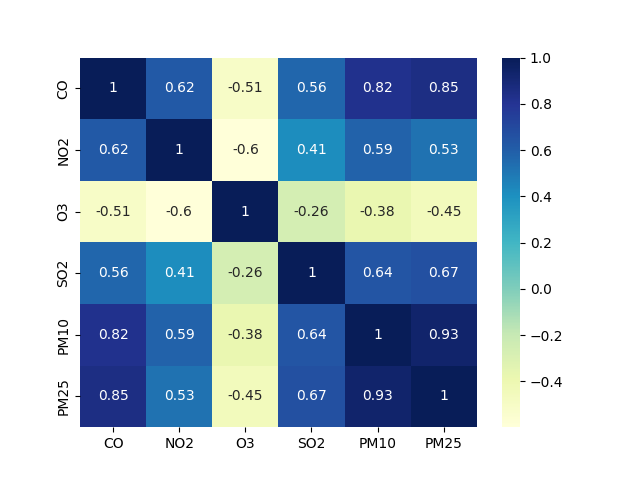
\includegraphics[width=120mm, height=90mm]{visualisations/corr_heatmaps/pollution_corr_heatmap.png}
\caption{Macierz korelacji metryk zanieczyszczenia powietrza}
\end{figure}

Macierz korelacji metryk zanieczyszczenia powietrza pokazuje wyraźną korelację między nimi. Szczególnie silnie skorelowane są oba rodzaje pyłów (PM25 i PM10) oraz tlenek węgla (CO). Słabiej, ale wciąż wyraźnie skorelowane z innymi metrykami są dwutlenki siarki (SO2) i azotu (NO2). Zaskakująca może być negatywna korelacja stężenia ozonu troposferycznego ze wszystkimi pozostałymi metrykami. Możliwe przyczyny tego zjawiska zostaną omówione w dalszej części analizy.

\begin{figure}[H]
\centering
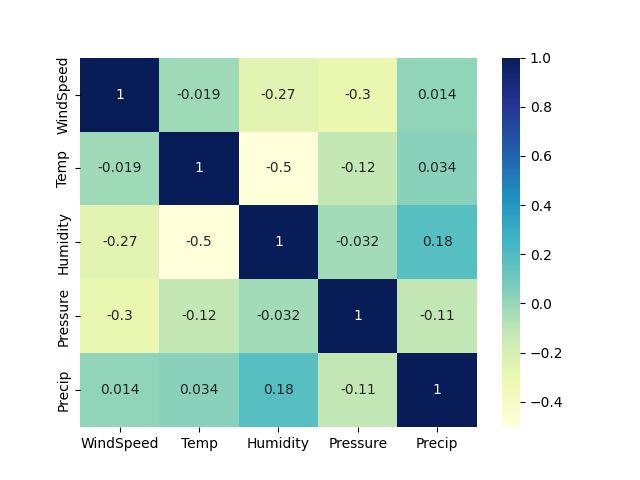
\includegraphics[width=120mm, height=90mm]{visualisations/corr_heatmaps/weather_corr_rolling_heatmap.png}
\caption{Macierz korelacji zmiennych pogodowych}
\end{figure}

Dla właściwego zinterpretowania zależności między zmiennymi pogodowymi a jakością powietrza istotna może się też okazać znajomość zależności między samymi zmiennymi pogodowymi. Macierz korelacji pokazuje tu wyraźną korelację ujemną między temperaturą a wilgotnością. Można też zauważyć słabsze korelacje: ujemne między ciśnieniem i wilgotnością a prędkością wiatru i dodatnią między wilgotnością a opadami. Należy wspomnieć, że mapę korelacji wykonano na podstawie danych uśrednionych w sześciogodzinnym oknie przesuwnym. Było to konieczne do właściwego uwzględnienia wielkości opadów, która jest podawana jedynie co 6 godzin. Kierunek wiatru pominięto ze względu na jego nieliniowy charakter.

\begin{figure}[H]
\centering
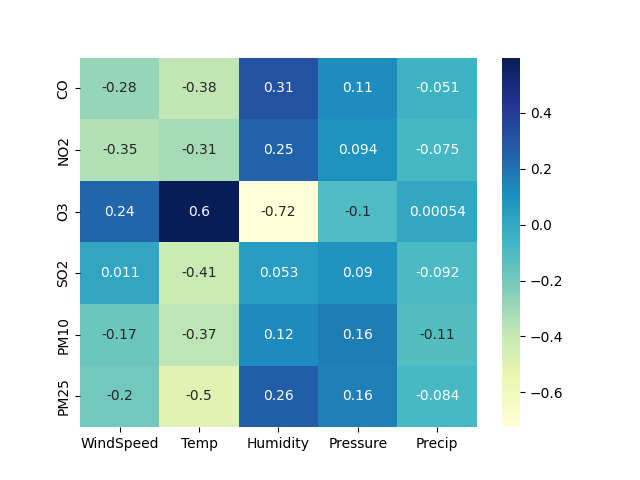
\includegraphics[width=120mm, height=90mm]{visualisations/corr_heatmaps/pollutionxweather_corr_heatmap.png}
\caption{Macierz korelacji zmiennych pogodowych z metrykami zanieczyszczenia powietrza}
\end{figure}

Następnie zbadano korelacje między zmiennymi pogodowymi a metrykami zanieczyszczenia powietrza. Z wyłączeniem ozonu, większość metryk jest pozytywnie skorelowana z wilogtnością i ciśnieniem oraz negatywnie z temperaturą i prędkością wiatru; korelacja z temperaturą jest szczególnie silna. Ozon wydaje się zachowywać dokładnie przeciwnie do wszystkich innych metryk.

Zależności te zostaną dokładniej zbadane w dalszej części analizy.

\subsubsection{Cykle czasowe}

Przed bliższą analizą zależności między zmiennymi pogodowymi a metrykami warto przyjrzeć się temu, jak wartości metryk zmieniają się w poszczególnych cyklach czasowych.

\begin{table}[H]
\centering
\begin{tabular}{|c|c|}
\hline
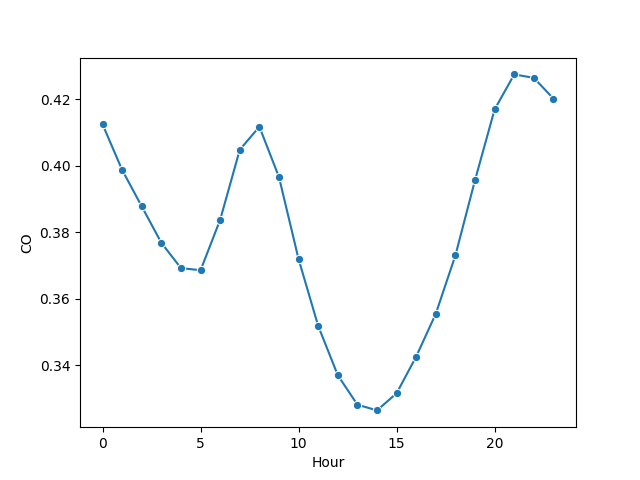
\includegraphics[width=80mm,height=60mm]{visualisations/cycles/hourly_CO.png}  & 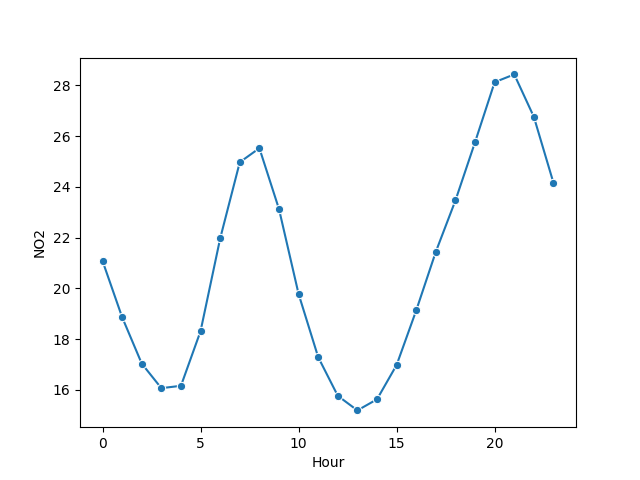
\includegraphics[width=80mm,height=60mm]{visualisations/cycles/hourly_NO2.png} \\ \hline
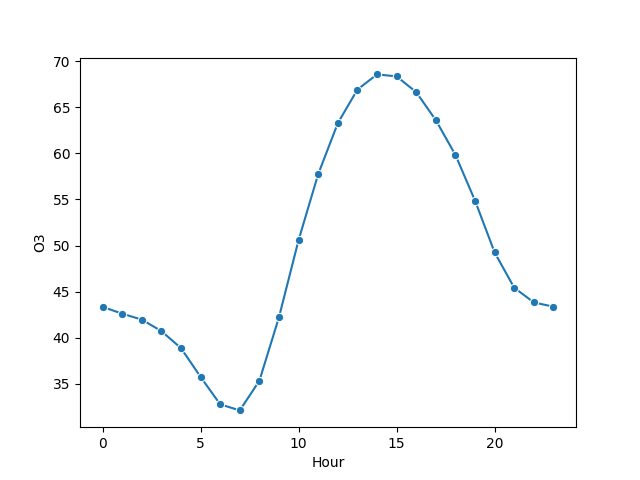
\includegraphics[width=80mm,height=60mm]{visualisations/cycles/hourly_O3.png}  & 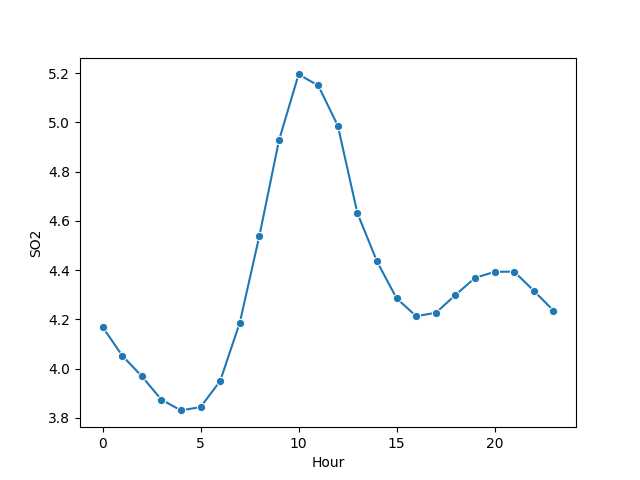
\includegraphics[width=80mm,height=60mm]{visualisations/cycles/hourly_SO2.png} \\ \hline
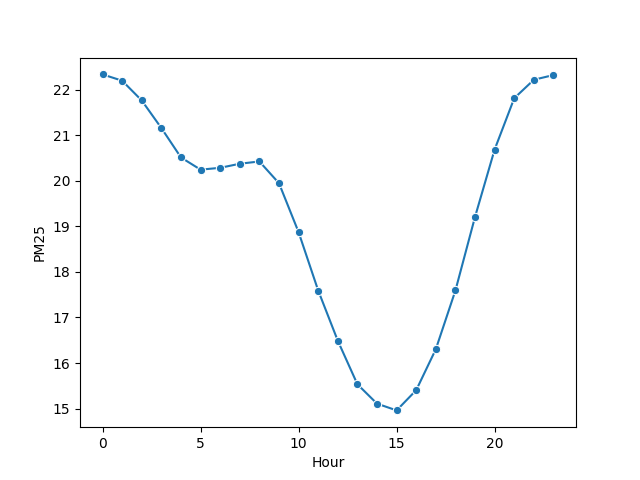
\includegraphics[width=80mm,height=60mm]{visualisations/cycles/hourly_PM25.png}  & 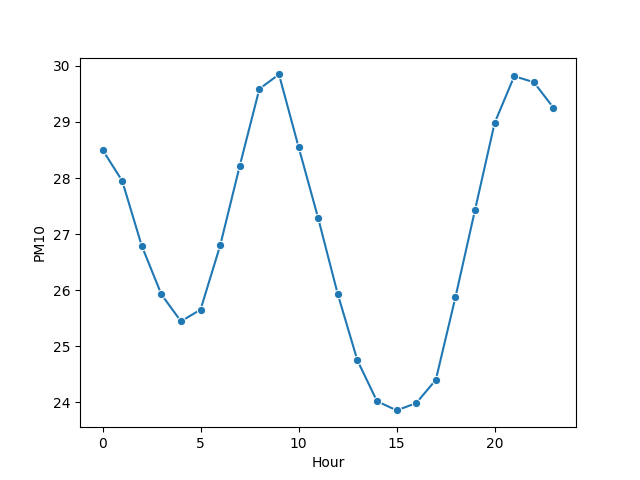
\includegraphics[width=80mm,height=60mm]{visualisations/cycles/hourly_PM10.png} \\ \hline
\end{tabular}
\caption{Zmiany metryk w cyklu dobowym}
\label{table:daily}
\end{table}

Tablica \ref{table:daily} zawiera wykresy średnich wartości poszczególnych metryk w zależności od godziny. Wykresy dla CO, NO2, PM25 i PM10 wyglądają podobnie: stężenia stopniowo maleją w godzinach nocnych, rosną od wczesnego ranka, gwałtownie maleją późnym rankiem i wczesnym popołudniem, a następnie znów rosną późnym popołudniem i wieczorem. Wykres dla O3 wygląda niemal dokładnie odwrotnie - minimum przypada na ranek, a maksimum na popołudnie. Z kolei stężenie SO2 osiągają maksimum około południa po czym gwałtownie spadają, nieznacznie rosną wieczorem, po czym znów spadają do minimum wczesnym rankiem.

Wyniki te mogą być zaskakujące. Ponieważ zanieczyszczenia są produktem ludzkiej aktywności, a aktywność ta jest najintesywniejsza za dnia, można by oczekiwać, że również stężenia zanieczyszczeń będą wtedy największe. Jednak z wybranych sześciu metryk aż cztery wykazują dokładnie przeciwne zachowanie, tj. dobowe minimum przypada na godziny dzienne, a maksimum na wczesną noc. Możliwym wyjaśnieniem takiego zachowania jest mechanizm tzw. inwersji temperatury, w ramach której w nocy tworzy się przy ziemi warstwa powietrza zimniejszego niż w warstwach wyższych, co "więzi" zanieczyszczenia blisko powierzchni. Za dnia natomiast, nagrzana ziemia ogrzewa również bezpośrednio się z nią stykającą warstwę powietrza, przez co powietrze to unosi się i rozwiewa cząstki zanieczyszczeń. Za dnia większa jest również średnia prędkość wiatru (wykres \ref{figure:wind_daily}), co także sprzyja rozwiewaniu się zanieczyszczeń.

\begin{figure}[H]
\centering
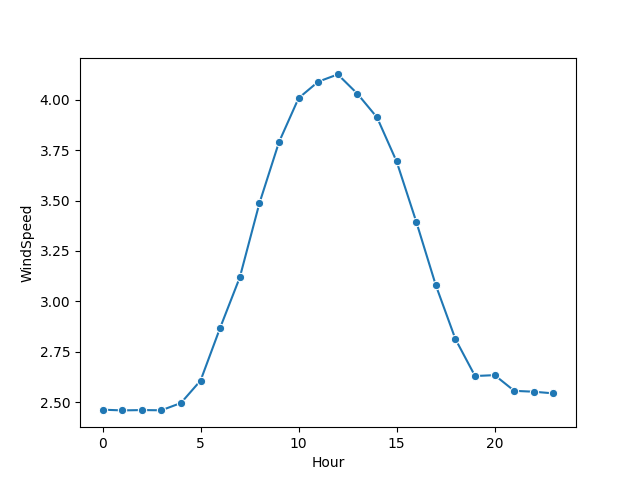
\includegraphics[width=120mm, height=90mm]{visualisations/weather_cycles/hourly_wind_speed.png}
\caption{Średnia prędkość wiatru w zależności od godziny}
\label{figure:wind_daily}
\end{figure}

Ten mechanizm, w połączeniu z dziennym cyklem ludzkiej aktywności dobrze tłumaczy zachowanie CO, NO2, PM25 i PM10: stężenia rosną późnym popołudniem, bo zmniejszanie się temperatury nakłada się na wciąż intensywną ludzką działalność. Następnie ze względu na mniejszą ludzką aktywność stężenia powoli spadają, aż do ranka, gdy nagły wzrost ludzkiej aktywności (wiele osób jedzie do pracy, szkoły; rozpoczynają pracę zakłady przemysłowe itp.) w połączeniu z wciąż jeszcze niską temperaturą powoduje nowy gwałtowny wzrost stężeń. Wreszcie za dnia efekt cieplejszego powietrza ponownie prowadzi do spadku stężeń.

Zachowanie się metryki O3 może się w tym kontekście wydawać paradoksalne, łatwo jest jednak je wytłumaczyć, jeśli weźmie się pod uwagę następujace fakty: 

\begin{itemize}
\item ozon nie jest generowany bezpośrednio przez ludzką działalność, lecz powstaje z innych, wytwarzanych przez ludzi substancji w naturalnie zachodzących reakcjach chemicznych; reakcje te zachodzą najintensywniej w obecności światła słonecznego i wysokiej temperatury
\item ozon troposferyczny jest niestabilny i rozpada się w reakcjach z m. in. tlenkami azotu, które również są emitowane przez człowieka
\end{itemize}

Biorąc to pod uwagę nie jest zaskakujące, że ozon, który powstaje w warunkach niesprzyjających wysokim koncentracjom innych zanieczyszczeń oraz rozpada się w kontakcie z nimi zachowuje się pod wieloma względami odwrotnie do nich.

Zachowanie ostatniej metryki, SO2, trudniej jest wytłumaczyć. Być może większa masa cząstek (w porównaniu z CO, O3 i NO2) sprawia, że różnice temperatur mają mniejszy wpływ na ich stężenia?

Dla lepszego zoobrazowania opisywanych relacji zestawiono wykresy dziennych cykli metryk z wykresem średnich temperatur w zależności od godziny (tabela \ref{table:daily_temp}). Warto zwrócić uwagę, jak zbliżone są kształty wykresów O3 i temperatury.

\begin{table}[H]
\centering
\begin{tabular}{|c|c|}
\hline
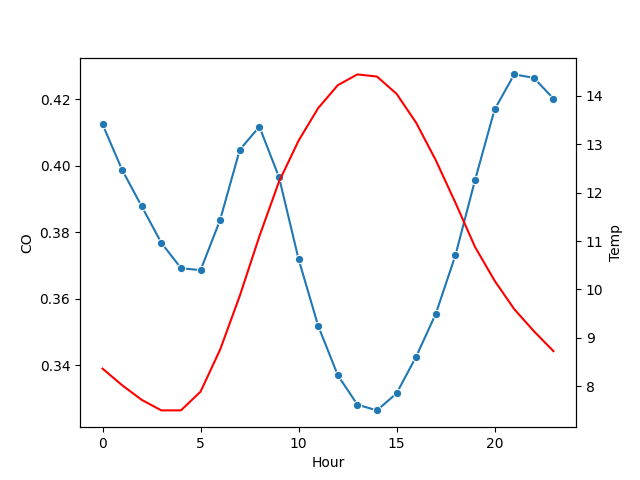
\includegraphics[width=80mm,height=60mm]{visualisations/cycles/hourly_CO_temp.png}  & 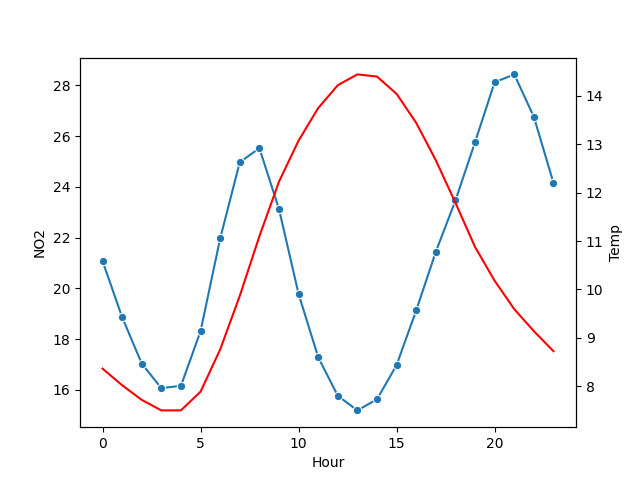
\includegraphics[width=80mm,height=60mm]{visualisations/cycles/hourly_NO2_temp.png} \\ \hline
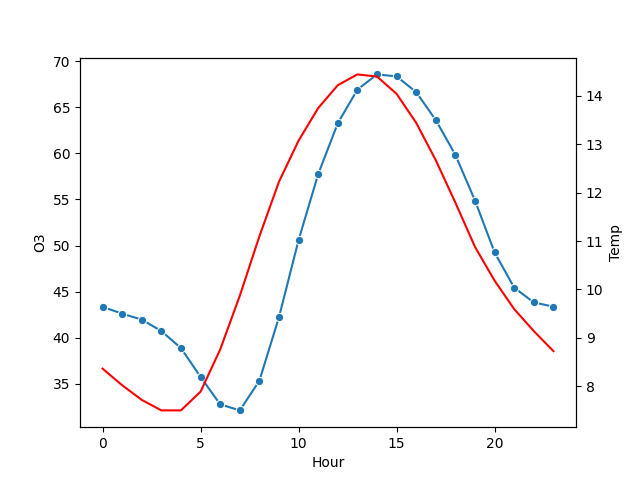
\includegraphics[width=80mm,height=60mm]{visualisations/cycles/hourly_O3_temp.png}  & 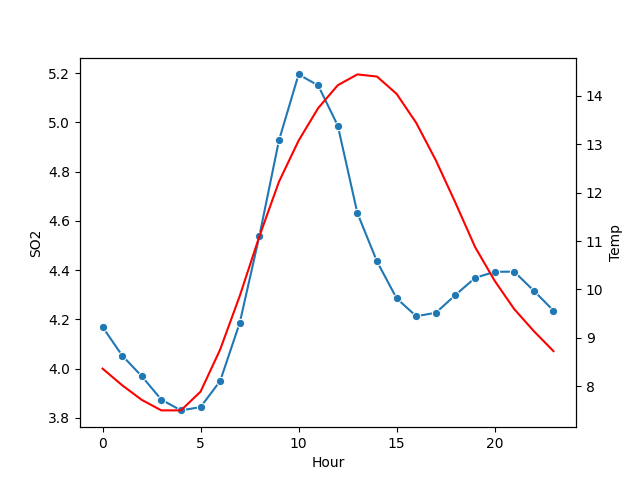
\includegraphics[width=80mm,height=60mm]{visualisations/cycles/hourly_SO2_temp.png} \\ \hline
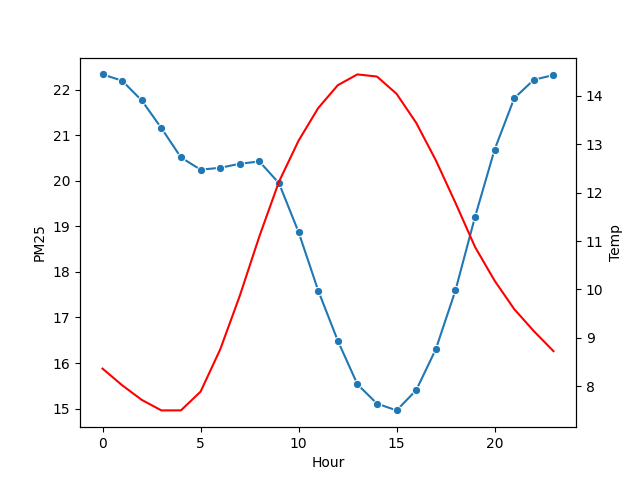
\includegraphics[width=80mm,height=60mm]{visualisations/cycles/hourly_PM25_temp.png}  & 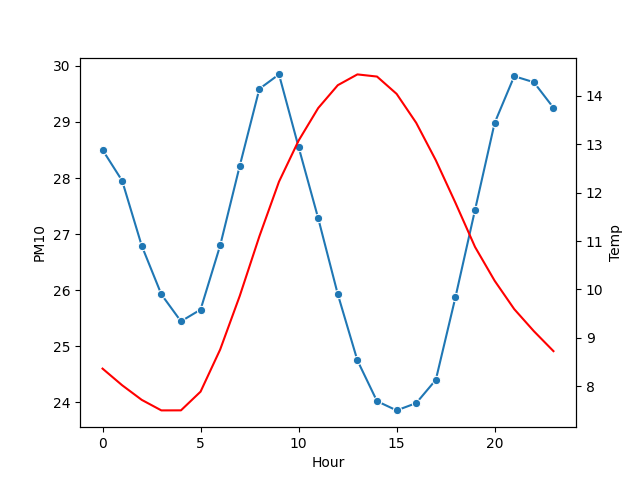
\includegraphics[width=80mm,height=60mm]{visualisations/cycles/hourly_PM10_temp.png} \\ \hline
\end{tabular}
\caption{Zmiany metryk w cyklu dobowym zestawione z temperaturą}
\label{table:daily_temp}
\end{table}

\begin{table}[H]
\centering
\begin{tabular}{|c|c|}
\hline
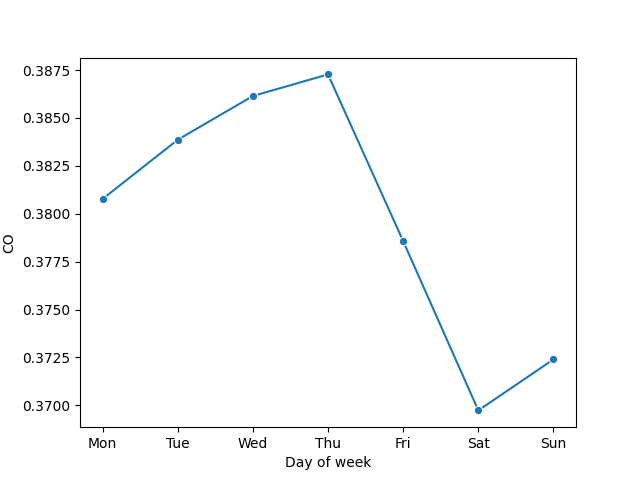
\includegraphics[width=80mm,height=60mm]{visualisations/cycles/weekly_CO.png}  & 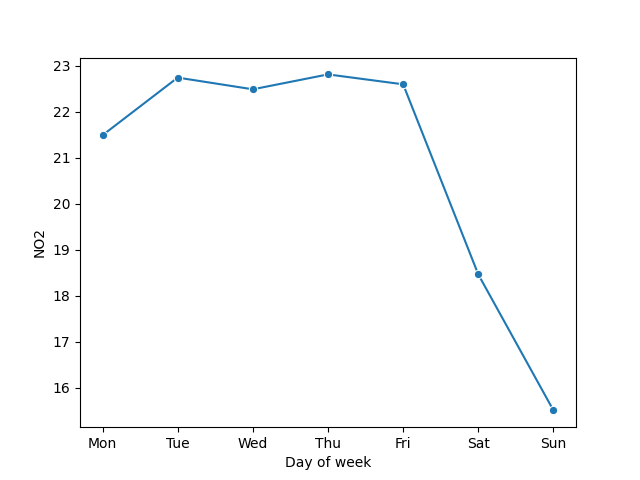
\includegraphics[width=80mm,height=60mm]{visualisations/cycles/weekly_NO2.png} \\ \hline
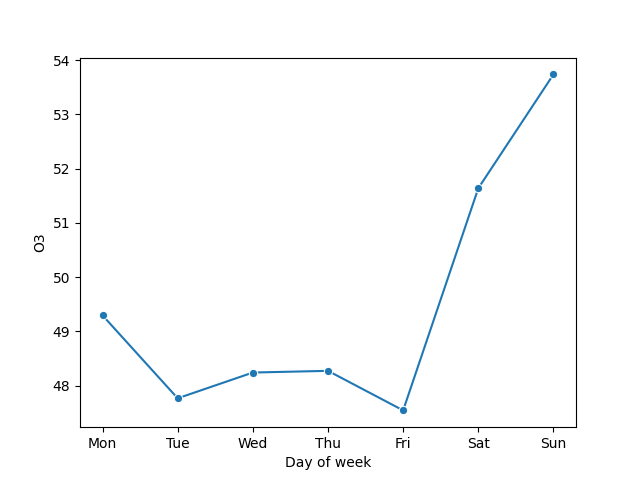
\includegraphics[width=80mm,height=60mm]{visualisations/cycles/weekly_O3.png}  & 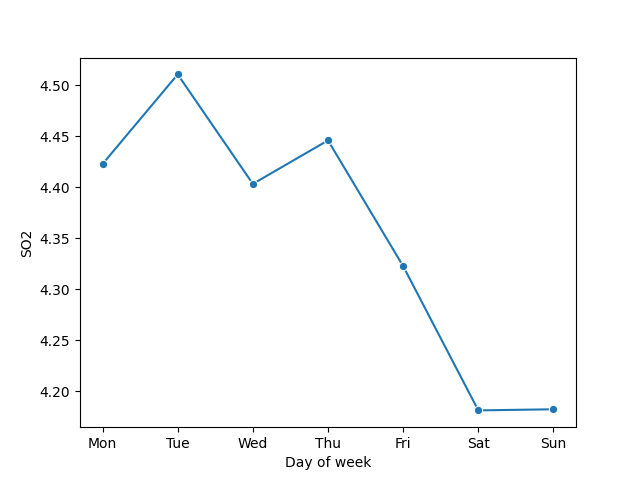
\includegraphics[width=80mm,height=60mm]{visualisations/cycles/weekly_SO2.png} \\ \hline
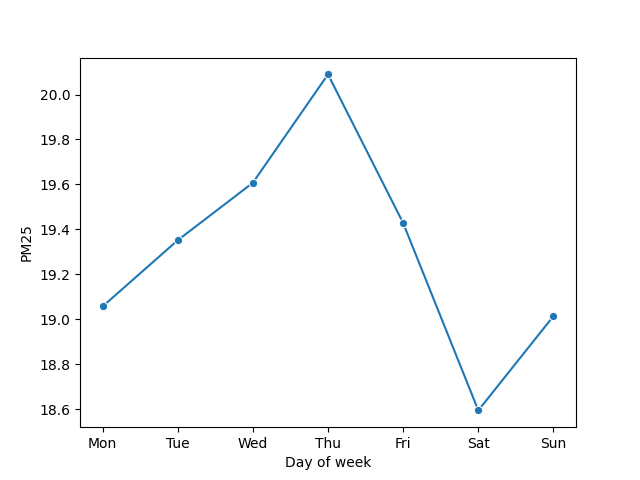
\includegraphics[width=80mm,height=60mm]{visualisations/cycles/weekly_PM25.png}  & 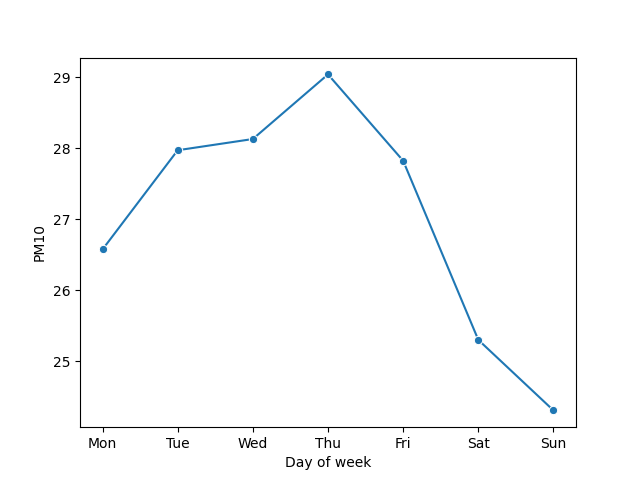
\includegraphics[width=80mm,height=60mm]{visualisations/cycles/weekly_PM10.png} \\ \hline
\end{tabular}
\caption{Zmiany metryk w cyklu tygodniowym}
\label{table:weekly}
\end{table}

Tablica \ref{table:weekly} zawiera wykresy średnich wartości poszczególnych metryk w zależności od dnia tygodnia. Ponieważ tydzień jest jednostką czasu wymyśloną przez ludzi, niezwiązaną z żadnym istotnym dla atmosfery naturalnym cyklem, można założyć że wszelkie zależności będą wynikać wyłącznie z działalności człowieka.

Kształty wykresów dla poszczególnych metryk różnią się, jednak łatwo można zauważyć wspólny element: stężenia są największe w dni robocze i spadają w weekendy. Wynika to zapewne z tego, że w weekendy nie funkcjonuje wiele instytucji i zakładów pracy, a co za tym idzie istnieje też mniejsza potrzeba poruszania się, zwłaszcza za pomocą wysokoemisyjnych środków transportu takich jak samochody. Wyjątkiem od tej ogólnej reguły jest, ponownie, ozon. Można przypuszczać, że cząsteczki ozonu trwają w atmosferze dłużej przy mniejszych stężeniach innych substancji, w reakcji z którymi mogły by się rozpaść. Z podobnych przyczyn czasem obserwuje się większe stężenia ozonu troposferycznego na terenach wiejskich niż miejskich. \cite{ozone_rural}

Tablica \ref{table:yearly} zawiera wykresy średnich wartości poszczególnych metryk w zależności od miesiąca. 

Wykresy dla większości metryk mają podobny kształt: wartości są największe zimą, z maximum w styczniu lub lutym, i najmniejsze latem, z minimum w czerwcu, lipcu lub sierpniu. Może to wynikać po części z opisanego wcześniej wpływu temperatury, jak i z większego zapotrzebowania na ogrzewanie zimą (co przekłada się pośrednio lub bezpośrednio na większe spalanie paliw kopalnych). Możliwe też, że zimą jest większy ruch samochodowy, gdyż pogoda zniechęca do poruszania się na pieszo lub rowerem. 

Ozon ponownie zachowuje się odwrotnie do pozostałych metryk.

\subsubsection{Zależności między zmiennymi i metrykami}
Na kolejnych wykresach przedstawiono zależnością między poszczególnymi zmiennych pogodowych i metrykami zanieczyszczenia powietrza. Na każdy wykres naniesiono linię regresji liniowej, która zazwyczaj nie jest adekwatnym modelem zależności, ale pomaga zwizualizować ogólny trend.

\begin{table}[H]
\centering
\begin{tabular}{|c|c|}
\hline
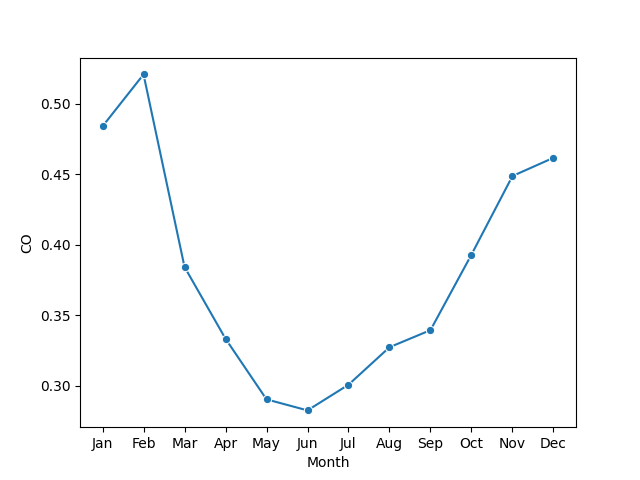
\includegraphics[width=80mm,height=60mm]{visualisations/cycles/monthly_CO.png}  & 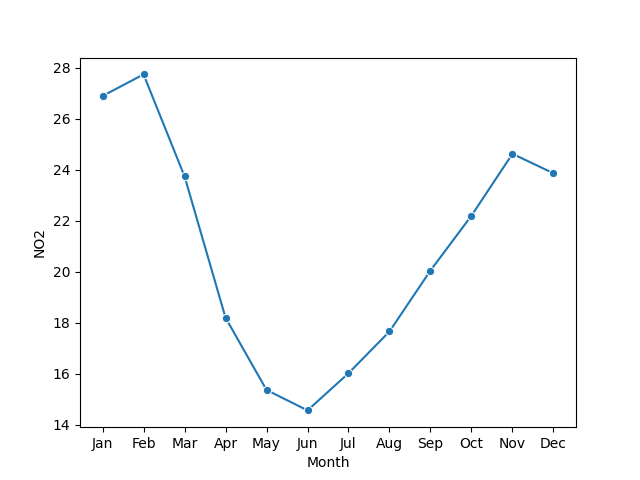
\includegraphics[width=80mm,height=60mm]{visualisations/cycles/monthly_NO2.png} \\ \hline
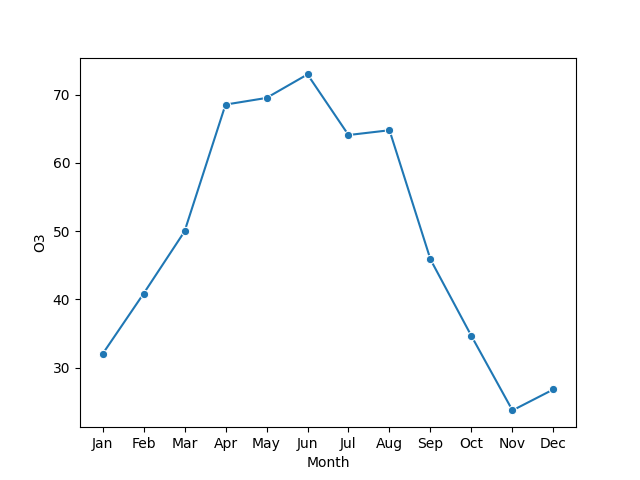
\includegraphics[width=80mm,height=60mm]{visualisations/cycles/monthly_O3.png}  & 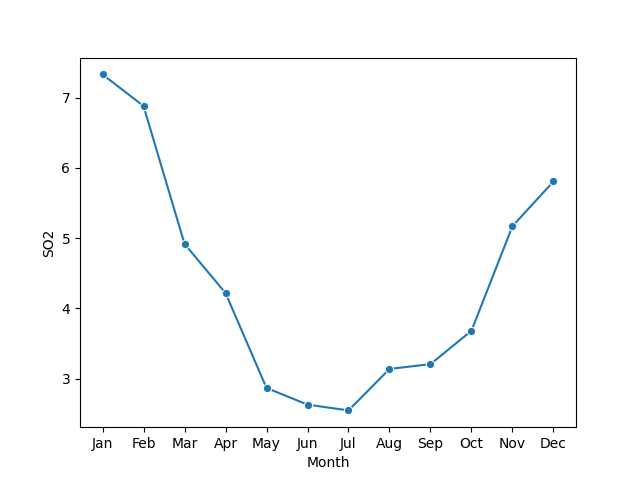
\includegraphics[width=80mm,height=60mm]{visualisations/cycles/monthly_SO2.png} \\ \hline
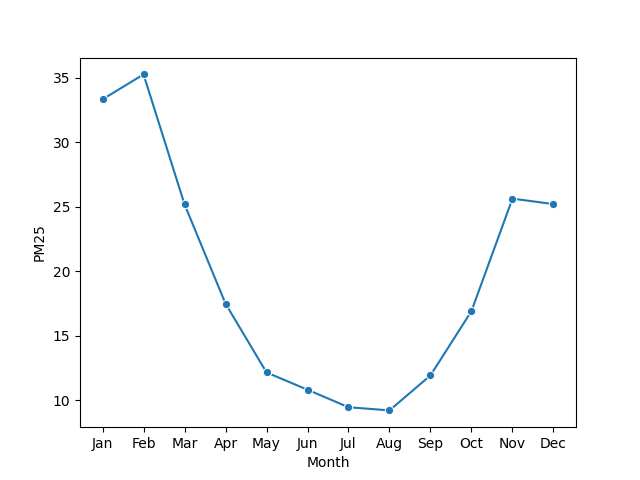
\includegraphics[width=80mm,height=60mm]{visualisations/cycles/monthly_PM25.png}  & 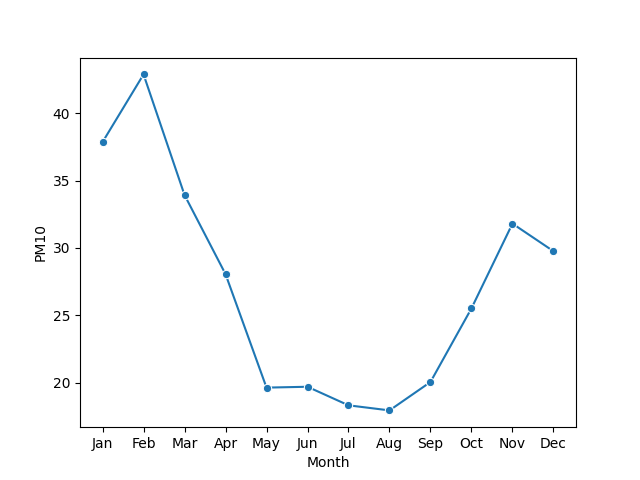
\includegraphics[width=80mm,height=60mm]{visualisations/cycles/monthly_PM10.png} \\ \hline
\end{tabular}
\caption{Zmiany metryk w cyklu rocznym}
\label{table:yearly}
\end{table}

\begin{table}[H]
\centering
\begin{tabular}{|c|c|}
\hline
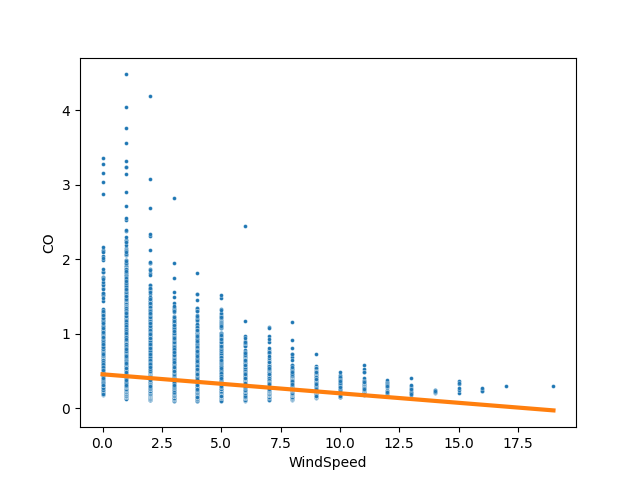
\includegraphics[width=80mm,height=60mm]{visualisations/corr_plots/WindSpeedxCO_scatter.png}  & 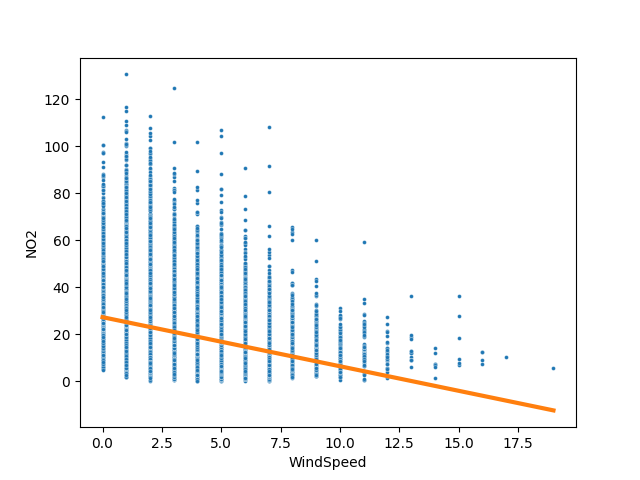
\includegraphics[width=80mm,height=60mm]{visualisations/corr_plots/WindSpeedxNO2_scatter.png} \\ \hline
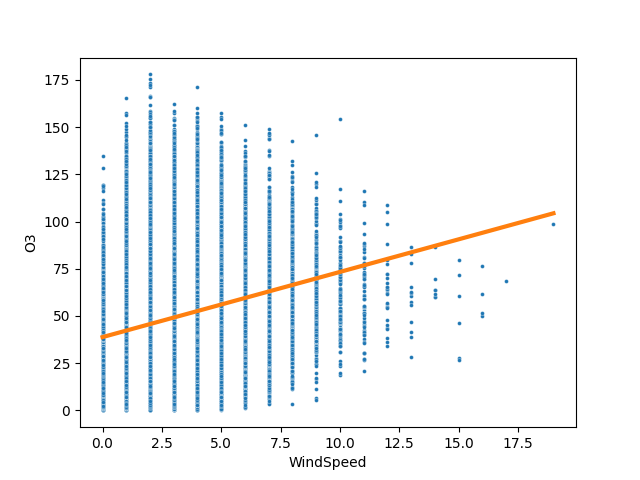
\includegraphics[width=80mm,height=60mm]{visualisations/corr_plots/WindSpeedxO3_scatter.png}  & 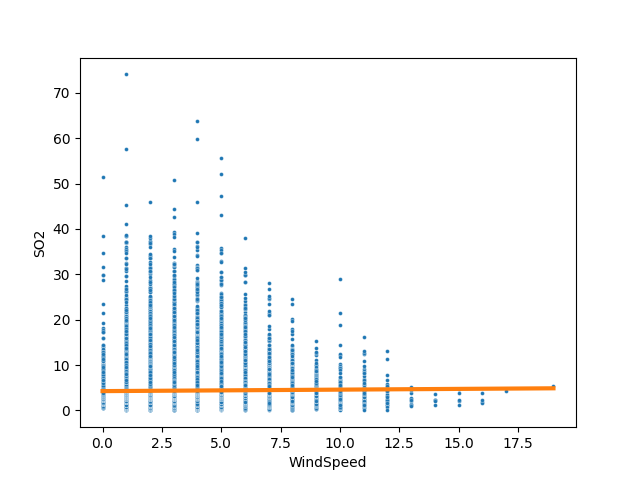
\includegraphics[width=80mm,height=60mm]{visualisations/corr_plots/WindSpeedxSO2_scatter.png} \\ \hline
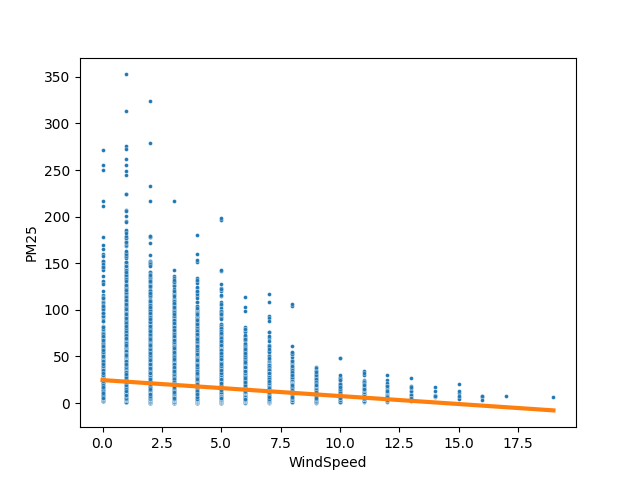
\includegraphics[width=80mm,height=60mm]{visualisations/corr_plots/WindSpeedxPM25_scatter.png}  & 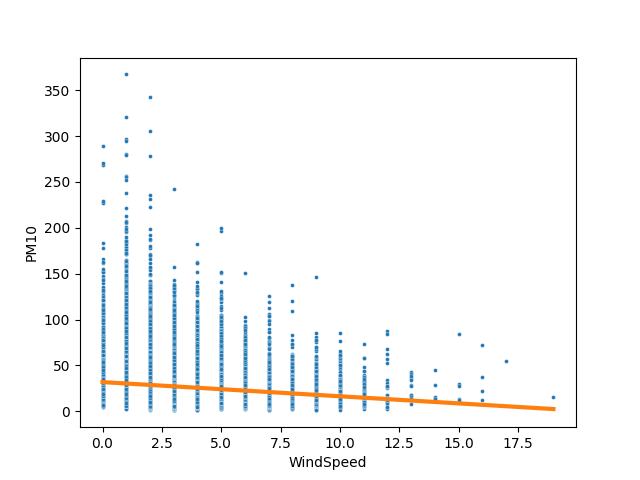
\includegraphics[width=80mm,height=60mm]{visualisations/corr_plots/WindSpeedxPM10_scatter.png} \\ \hline
\end{tabular}
\caption{Zależności metryk od prędkości wiatru}
\label{table:wind_speed}
\end{table}


\begin{table}[H]
\centering
\begin{tabular}{|c|c|}
\hline
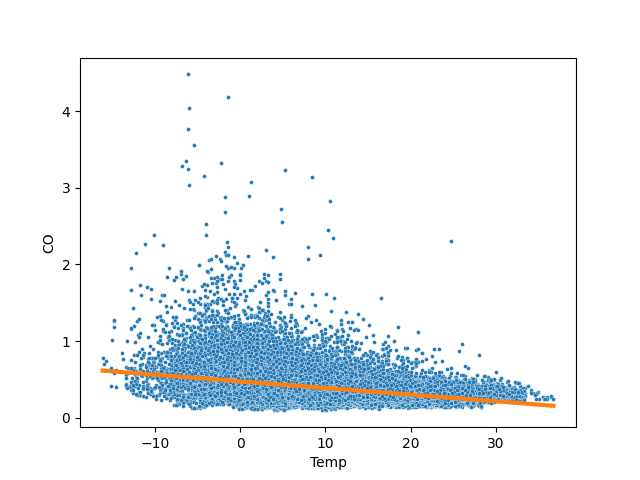
\includegraphics[width=80mm,height=60mm]{visualisations/corr_plots/TempxCO_scatter.png}  & 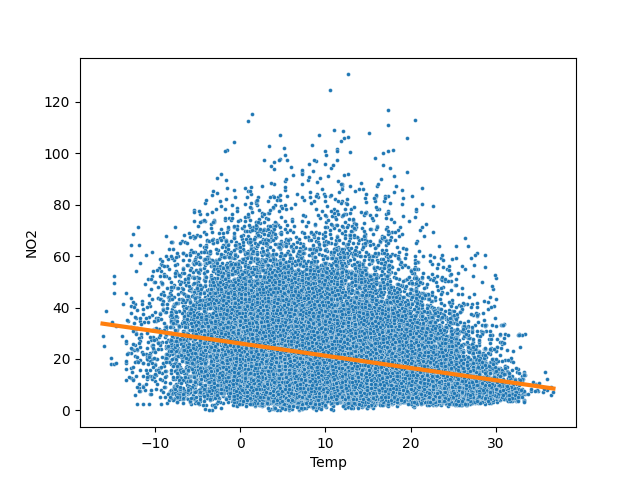
\includegraphics[width=80mm,height=60mm]{visualisations/corr_plots/TempxNO2_scatter.png} \\ \hline
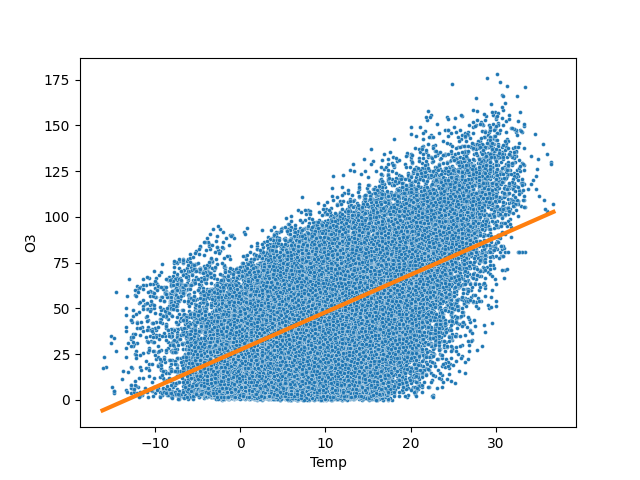
\includegraphics[width=80mm,height=60mm]{visualisations/corr_plots/TempxO3_scatter.png}  & 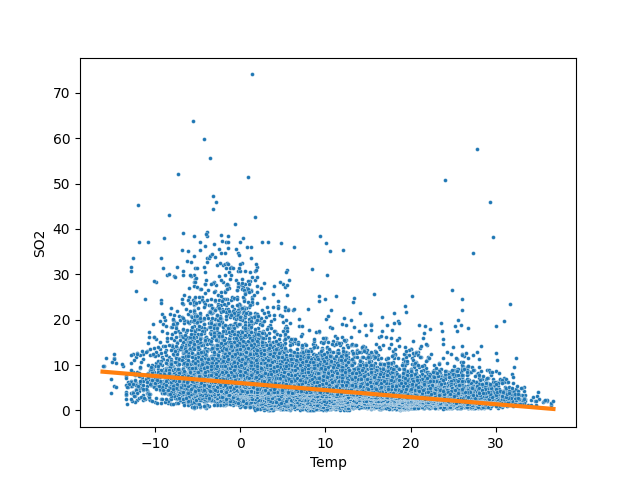
\includegraphics[width=80mm,height=60mm]{visualisations/corr_plots/TempxSO2_scatter.png} \\ \hline
\includegraphics[width=80mm,height=60mm]{visualisations/corr_plots/TempxPM25_scatter.png}  & \includegraphics[width=80mm,height=60mm]{visualisations/corr_plots/TempxPM10_scatter.png} \\ \hline
\end{tabular}
\caption{Zależności metryk od temperatury}
\label{table:temperature}
\end{table}

\begin{table}[H]
\centering
\begin{tabular}{|c|c|}
\hline
\includegraphics[width=80mm,height=60mm]{visualisations/corr_plots/HumidityxCO_scatter.png}  & \includegraphics[width=80mm,height=60mm]{visualisations/corr_plots/HumidityxNO2_scatter.png} \\ \hline
\includegraphics[width=80mm,height=60mm]{visualisations/corr_plots/HumidityxO3_scatter.png}  & \includegraphics[width=80mm,height=60mm]{visualisations/corr_plots/HumidityxSO2_scatter.png} \\ \hline
\includegraphics[width=80mm,height=60mm]{visualisations/corr_plots/HumidityxPM25_scatter.png}  & \includegraphics[width=80mm,height=60mm]{visualisations/corr_plots/HumidityxPM10_scatter.png} \\ \hline
\end{tabular}
\caption{Zależności metryk od wilgotności}
\label{table:humidity}
\end{table}

\begin{table}[H]
\centering
\begin{tabular}{|c|c|}
\hline
\includegraphics[width=80mm,height=60mm]{visualisations/corr_plots/PressurexCO_scatter.png}  & \includegraphics[width=80mm,height=60mm]{visualisations/corr_plots/PressurexNO2_scatter.png} \\ \hline
\includegraphics[width=80mm,height=60mm]{visualisations/corr_plots/PressurexO3_scatter.png}  & \includegraphics[width=80mm,height=60mm]{visualisations/corr_plots/PressurexSO2_scatter.png} \\ \hline
\includegraphics[width=80mm,height=60mm]{visualisations/corr_plots/PressurexPM25_scatter.png}  & \includegraphics[width=80mm,height=60mm]{visualisations/corr_plots/PressurexPM10_scatter.png} \\ \hline
\end{tabular}
\caption{Zależności metryk od ciśnienia atmosferycznego}
\label{table:pressure}
\end{table}

\begin{table}[H]
\centering
\begin{tabular}{|c|c|}
\hline
\includegraphics[width=80mm,height=60mm]{visualisations/corr_plots/precipxCO_scatter.png}  & \includegraphics[width=80mm,height=60mm]{visualisations/corr_plots/precipxNO2_scatter.png} \\ \hline
\includegraphics[width=80mm,height=60mm]{visualisations/corr_plots/precipxO3_scatter.png}  & \includegraphics[width=80mm,height=60mm]{visualisations/corr_plots/precipxSO2_scatter.png} \\ \hline
\includegraphics[width=80mm,height=60mm]{visualisations/corr_plots/precipxPM25_scatter.png}  & \includegraphics[width=80mm,height=60mm]{visualisations/corr_plots/precipxPM10_scatter.png} \\ \hline
\end{tabular}
\caption{Zależności metryk od wielkości opadów}
\label{table:precipitation}
\end{table}

Wykresy zależności potwierdzają intuicje uzyskane z analizy macierzy korelacji, pozwalają też jednak na wyciągnięcie bardziej szczegółowych wniosków.

Wysoka prędkość wiatru zdaje się nakładać pewnego rodzaju górny limit na stężenia zanieczyszczeń. Nie wydaje się to zaskakujące - silny wiatr rozprasza zanieczyszczenia na większym obszarze, tym samym zmniejszając ich stężenia w mieście. Ciekawe jest to, że największe stężenia są osiągane przy słabym wietrze, nie zaś przy jego całkowitym braku. Możliwe, że minimalny wiatr jest potrzebny, aby znaczniejsze ilości zanieczyszczeń dotarły do stacji pomiarowej. Ozon ponownie zachowuje się inaczej niż pozostałe substancje: w jego przypadku szybki wiatr zdaje się uniemożliwiać zarówno bardzo wysokie, jak i bardzo niskie stężenia.

Wykresy zależności metryk od temperatury pokrywają się z wcześniejszymi wnioskami: ozon jest silnie pozytywnie skorelowany z temperaturą, pozostałe metryki wykazują słabszą zależność negatywną.

Większość metryk, z wyjątkiem ozonu, wykazuje nieznaczną pozytywną korelację z wilgotnością. Jako że wilgotność wykazuje negatywną korelację z temperaturą, można przypuszczać że za tą zależnością stoi w znacznym stopniu wpływ temperatury, a nie samej wilgotności.

Większość metryk wykazuje pozytywną korelację z ciśnieniem, a szczególnie wysokie stężenia zdarzają się głównie przy wysokim ciśnieniu (szczególnie w przypadku pyłów i tlenku węgla). Ozon natomiast wykazuje najwyższe wartości przy średnim ciśnieniu, a jego stężenia spadają spadają gdy ciśnienie zbliża się do wartości ekstremalnych.

Podobnie jak w przypadku prędkości wiatru, silne opady wydają się nie dopuszczać do utrzymywania się wysokich stężeń zanieczyszczeń.

Ze względu na nieliniowość kierunku wiatru, zależności między nim a metrykami zanieczyszczenia powietrza przedstawiono na wykresach pudełkowych. NULL oznacza brak wiatru.

\begin{figure}[H]
\centering
\includegraphics[width=100mm, height=75mm]{visualisations/wind_dir_pollution_patterns/wind_dir_CO.png}
\caption{Zależność stężenia CO od kierunku wiatru}
\end{figure}

\begin{figure}[H]
\centering
\includegraphics[width=100mm, height=75mm]{visualisations/wind_dir_pollution_patterns/wind_dir_NO2.png}
\caption{Zależność stężenia NO2 od kierunku wiatru}
\end{figure}

\begin{figure}[H]
\centering
\includegraphics[width=100mm, height=75mm]{visualisations/wind_dir_pollution_patterns/wind_dir_O3.png}
\caption{Zależność stężenia O3 od kierunku wiatru}
\end{figure}

\begin{figure}[H]
\centering
\includegraphics[width=100mm, height=75mm]{visualisations/wind_dir_pollution_patterns/wind_dir_SO2.png}
\caption{Zależność stężenia SO2 od kierunku wiatru}
\end{figure}

\begin{figure}[H]
\centering
\includegraphics[width=100mm, height=75mm]{visualisations/wind_dir_pollution_patterns/wind_dir_PM25.png}
\caption{Zależność stężenia PM25 od kierunku wiatru}
\end{figure}

\begin{figure}[H]
\centering
\includegraphics[width=100mm, height=75mm]{visualisations/wind_dir_pollution_patterns/wind_dir_PM10.png}
\caption{Zależność stężenia PM10 od kierunku wiatru}
\end{figure}

Pomijając ozon, największe stężenia zanieczyszczeń występują przy bezwietrznej pogodzie (co nie jest zaskakujące, biorąc pod uwagę wykres zależności od prędkości wiatru) oraz przy wietrze południowo-wschodnim, najmniejsze zaś przy wietrze północno-zachodnim.

\subsubsection{Bonus - wpływ kierunku wiatru w zależności od położenia na terenie miasta}

W ramach analizy zależności postanowiłem dodatkowo sprawdzić, jak zależność stężeń zanieczyszczeń od kierunku wiatru wygląda w danych z innej stacji pomiarowej, znajdującej się w innej części Wrocławia (na aleji Wiśniowej, a zatem po przeciwnej stronie centrum niż stacja na wybrzeżu Conrada). Jeśli zależności będą wyglądały inaczej, będzie to stanowiło potwierdzenie, że uzyskane rezultaty wynikają z położenia względem największych źródeł zanieczyszczeń na terenia centrum miasta i jego okolic. Jeśli zaś będą wyglądały podobnie, będzie można to uznać za poszlakę, że różnice w jakości powietrza w zależności od kierunku wiatru wynikają z innych czynników, np. wpływu kierunku wiatru na inne zmienne pogodowe lub źródeł zanieczyszczeń w oddaleniu od centrum. Z powodu niedostatku danych z alternatywnej stacji pomiarowej, test zostanie przeprowadzony tylko dla trzech metryk: CO, NO2 i PM25. Wyniki tego testu są tu zamieszczane w formie ciekawostki i nie zostaną uwzględnione w ostatecznie tworzonym modelu.

\begin{figure}[H]
\centering
\includegraphics[width=100mm, height=75mm]{visualisations/wind_dir_pollution_alt_patterns/wind_dir_CO.png}
\caption{Zależność stężenia CO od kierunku wiatru - stacja al. Wiśniowa}
\end{figure}

\begin{figure}[H]
\centering
\includegraphics[width=100mm, height=75mm]{visualisations/wind_dir_pollution_alt_patterns/wind_dir_NO2.png}
\caption{Zależność stężenia NO2 od kierunku wiatru - stacja al. Wiśniowa}
\end{figure}

\begin{figure}[H]
\centering
\includegraphics[width=100mm, height=75mm]{visualisations/wind_dir_pollution_alt_patterns/wind_dir_PM25.png}
\caption{Zależność stężenia PM25 od kierunku wiatru - stacja al. Wiśniowa}
\end{figure}

Dla danych z alternatywnej stacji pomiarowej zależności wyglądają podobnie - zanieczyszczeń jest najwięcej przy wietrze południowo-wschodnim, a najmniej przy północno-zachodnim. Sugeruje to, że położenie względem źródeł zanieczyszczeń na terenie miasta nie jest głównym czynnikiem wpływającym na zależność zanieczyszczenia od kierunku wiatru.

\section{Eksperymenty modelowania}

Podjęta zostanie próba uzyskania modeli przewidujących wartości metryk zanieczyszczenia powietrza na podstawie wybranych zmiennych. Pierwsze kilka eksperymentów zostanie przeprowadzonych dla wybranej pojedynczej metryki (CO). Następnie wybrane metody zostaną też przetestowane dla pozostałych metryk. W ramach dwóch ostatnich ekseprymentów podjęta zostanie też próba stworzenia modeli wykorzystujących wybrane podzbiory zbioru zmiennych. Wypróbowane zostaną też dwa sposoby podziału zbioru danych na zbiór treningowy i testowy. Pierwszym sposobem jest podział losowy, który może odzwierciedlać sytuację, w której staramy się uzupełnić niepełny zbiór danych dotyczących jakości powietrza na podstawie danych dostępnych. Drugim sposobem będzie użycie jako zbioru testowego ostatniego roku dostępnych pomiarów - będzie to odzwierciedlać sytuację w której staramy się przewidzieć jakość powietrza obecnie lub w bliskiej przyszłości, na podstawie dostępnych już lub przewidywanych danych pogodowych. 
Jako główną metrykę oceny jakości modeli wykorzystano pierwiastek błędu średniokwadratowego. Przy niektórych testach podano też współczynnik determinacji R\textsuperscript{2}, czyli miara proporcji zmienności zmiennej zależnej, którą można przewidzieć na podstawie zmiennych niezależnych; wartości R\textsuperscript{2} przybierają wartości nie większe od 1 (gdzie 1 oznacza perfekcyjną predykcje). Miara ta jest wygodniejsza do porównywania modeli przewidująych poszczególne metryki, gdyż jej wartość, w przeciwieństwie do pierwiastka błędu średniokwadratowego, nie zależy od skali wartości docelowych.

\subsection{Eksperyment 1: regresja liniowa}

Jako pierwszy model, dla metryki CO, została zastosowana regresja liniowa z wykorzystaniem metody najmniejszych kwadratów. Metoda ta została wybrana głównie ze względu na swoją prostotę. Jej wyniki mogą posłużyć za podstawę do oceny bardziej zaawansowanych algorytmów.

Testy przeprowadzono dla obu sposobów podziału zbioru danych, z i bez uwzględniania zmiennych czasowych, tzn. godziny, dnia tygodnia i miesiąca jako zmiennych kategorycznych. Przy uwzględnieniu zmiennych czasowych poprzestano na regresji drugiego stopnia ze względu na bardzo dużą liczbę parametrów modelu dla wyższych stopni. Przy losowym podziale zbioru podział wykonywano po pięć razy, po czym obliczono uśredniony błąd.

\begin{table}[H]
\centering
\begin{tabular}{|c|cc|cc|}
\hline
Podział         & \multicolumn{2}{c|}{Losowy}        & \multicolumn{2}{c|}{Czasowy}       \\ \hline
Zmienne czasowe & \multicolumn{1}{c|}{Tak}   & Nie   & \multicolumn{1}{c|}{Tak}   & Nie   \\ \hline
1               & \multicolumn{1}{c|}{0.163} & 0.172 & \multicolumn{1}{c|}{0.135} & 0.138 \\ \hline
2               & \multicolumn{1}{c|}{42.78} & 0.158 & \multicolumn{1}{c|}{0.127} & 0.131 \\ \hline
3               & \multicolumn{1}{c|}{}      & 0.157 & \multicolumn{1}{c|}{}      & 0.131 \\ \hline
\end{tabular}
\caption{Pierwiastek błędów średniokwadratowych dla regresji metodą najmniejszych kwadratów}
\label{table:linear_results}
\end{table}

 Jak widać, uwzględnienie zmiennych czasowych istotnie poprawia wyniki. Wyniki są również wyraźnie lepsze przy podziale zbioru danych na bazie czasu niż przy podziałach losowych. Warto też zauważyć nieporównywalnie wysoki błąd dla modelu z losowym podziałem i uwzględnieniem zmiennych czasowych stopnia drugiego; może to wskazywać na bardzo duży overfitting.

\subsection{Eksperyment 2: algorytmy oparte na drzewach}

W kolejnym eksperymencie do tego samego problemu zostanie zastosowana metoda drzew decyzyjnych. Polega ona na zbudowaniu na podstawie danych treningowych drzewa binarnego, w którym każdy węzeł wewnętrzny zawiera warunek. Przy predykcji wektor zmiennych jest przekazywany do lewego lub prawego dziecka w zależności od tego, czy warunek jest spełniony czy nie, aż trafi do liścia; warunki zaś są dobierane tak, by na każdym kroku maksymalnie zmniejszyć wariancję zbiorów utworzonych przez podział zbioru treningowego. Liście drzewa zawierają konkretną predykcję, wyznaczaną zazwyczaj jako średnia wartości ze zbioru treningowego. Drzewa decyzyjne mają tendencję do overfittingu; ze względu na to zostaną wypróbowane różne limity głębokości drzewa.

Drzewo decyzyjne może sprawdzić się w tym problemie ze względu na dużą liczbę zmiennych kategorycznych i nieliniową naturę niektórych zależności (zwłaszcza tych związanych z czasem).

\begin{table}[H]
\centering
\begin{tabular}{|c|cc|cc|}
\hline
Podział         & \multicolumn{2}{c|}{Losowy}        & \multicolumn{2}{c|}{Czasowy}       \\ \hline
Zmienne czasowe & \multicolumn{1}{c|}{Tak}   & Nie   & \multicolumn{1}{c|}{Tak}   & Nie   \\ \hline
n=3             & \multicolumn{1}{c|}{0.169} & 0.169 & \multicolumn{1}{c|}{0.140} & 0.140 \\ \hline
n=4             & \multicolumn{1}{c|}{0.165} & 0.165 & \multicolumn{1}{c|}{0.137} & 0.137 \\ \hline
n=5             & \multicolumn{1}{c|}{0.159} & 0.161 & \multicolumn{1}{c|}{0.140} & 0.138 \\ \hline
n=6             & \multicolumn{1}{c|}{0.154} & 0.158 & \multicolumn{1}{c|}{0.143} & 0.148 \\ \hline
n=7             & \multicolumn{1}{c|}{0.151} & 0.156 & \multicolumn{1}{c|}{0.155} & 0.152 \\ \hline
n=8             & \multicolumn{1}{c|}{0.148} & 0.155 & \multicolumn{1}{c|}{0.157} & 0.156 \\ \hline
n=9             & \multicolumn{1}{c|}{0.150} & 0.153 & \multicolumn{1}{c|}{0.163} & 0.179 \\ \hline
\end{tabular}
\caption{Pierwiastek błędów średniokwadratowych dla regresji metodą drzew decyzyjnych, wartość n to maksymalna głębokość drzewa}
\label{table:tree_results}
\end{table}

Można zauważyć, że przy podziale losowym model sprawdza się gorzej dla mniejszej głębokości, ale lepiej dla większej. Być może losowy podział sprawia, że zbiory treningowe i testowe są do siebie bardziej podobne, przez co overfitting jest mniejszym zagrożeniem. Widać też, że uwzględnienie zmiennych czasowych nie zawsze poprawia wynik.

Nieco bardziej zaawansowaną metodą wykorzystującą drzewa decyzyjne jest las losowy. Las losowy stanowi rozwiązanie problemu niestabilności i tendencji do overfittingu drzew losowych. W ramach algorytmu tworzonych jest wiele drzew o losowych parametrach, a ostateczna predykcja jest średnią predykcji poszczególnych drzew.

\begin{table}[H]
\centering
\begin{tabular}{|c|cc|cc|}
\hline
Podział         & \multicolumn{2}{c|}{Losowy}        & \multicolumn{2}{c|}{Czasowy}       \\ \hline
Zmienne czasowe & \multicolumn{1}{c|}{Tak}   & Nie   & \multicolumn{1}{c|}{Tak}   & Nie   \\ \hline
n=3             & \multicolumn{1}{c|}{0.166} & 0.166 & \multicolumn{1}{c|}{0.138} & 0.139 \\ \hline
n=4             & \multicolumn{1}{c|}{0.161} & 0.161 & \multicolumn{1}{c|}{0.135} & 0.134 \\ \hline
n=5             & \multicolumn{1}{c|}{0.154} & 0.157 & \multicolumn{1}{c|}{0.133} & 0.133 \\ \hline
n=6             & \multicolumn{1}{c|}{0.150} & 0.153 & \multicolumn{1}{c|}{0.133} & 0.137 \\ \hline
n=7             & \multicolumn{1}{c|}{0.144} & 0.150 & \multicolumn{1}{c|}{0.132} & 0.142 \\ \hline
n=8             & \multicolumn{1}{c|}{0.140} & 0.148 & \multicolumn{1}{c|}{0.133} & 0.145 \\ \hline
n=9             & \multicolumn{1}{c|}{0.136} & 0.146 & \multicolumn{1}{c|}{0.133} & 0.151 \\ \hline
\end{tabular}
\caption{Pierwiastek błędów średniokwadratowych dla regresji metodą lasu losowego}
\label{table:forest_results}
\end{table}

Las losowy osiąga nieco lepsze wyniki niż zwykłe drzewa decyzyjne. Można zauważyć, że najlepsze wyniki są osiągane dla wyższych głębokości niż dla drzew decyzyjnych; potwierdza to, że las losowy jest bardziej odporny na overfitting. Nie widać tu też sytuacji, w których uwzględnienie danych czasowych pogarsza wynik, co świadczy o większej stabilności metody.

Dla podziału losowego metody oparte na drzewach są w stanie osiagać nieco lepsze rezultaty niż regresja liniowa. Dla podziału czasowego jednak nie uzyskano wyniku lepszego niż najlepszy wynik regresji liniowej.

\subsection{Eksperyment 3: porównanie wybranych modeli dla poszczególnych metryk}

\begin{table}[H]
\centering
\begin{tabular}{|c|c|c|c|c|c|c|}
\hline
         & CO    & NO2   & O3    & SO2  & PM25  & PM10  \\ \hline
Linear-1 & 0.135 & 12.27 & 16.61 & 2.79 & 12.17 & 16.6  \\ \hline
Linear-2 & 0.127 & 12.32 & 14.8  & 2.63 & 11    & 15.11 \\ \hline
Forest-7 & 0.132 & 12.3  & 17.7  & 2.77 & 12.3  & 15.9  \\ \hline
STD      & 0.2   & 14.41 & 30.38 & 3.54 & 18.33 & 20.34 \\ \hline
\end{tabular}
\caption{Pierwiasteki błędów średniokwadratowych dla poszczególnych metod i metryk, odchylenie standardowe dla porównania}
\label{table:general_results}
\end{table}

\begin{table}[H]
\centering
\begin{tabular}{|c|c|c|c|c|c|c|}
\hline
          & CO   & NO2 & O3   & SO2  & PM25 & PM10 \\ \hline
Linear-1 & 0.24 & 0.3 & 0.7  & 0.12 & 0.25 & 0.18 \\ \hline
Linear-2 & 0.34 & 0.4 & 0.76 & 0.22 & 0.39 & 0.32 \\ \hline
Forest-7 & 0.27 & 0.3 & 0.67 & 0.12 & 0.24 & 0.25 \\ \hline
\end{tabular}
\caption{Wartości R\textsuperscript{2} dla poszczególnych metod i metryk}
\label{table:general_results_r2}
\end{table}

Dla czasowego podziału zbioru i z uwzględnieniem zmiennych czasowych przeprowadzono testy trzech modeli: regresji liniowej pierwszego stopnia (Linear-1), regresji liniowej drugiego stopnia (Linear-2) oraz lasu losowego o głębokości 7 (Forest-7). 

W większości przypadków Linear-2 jest najlepszym z trzech modeli. Patrząc na wartości R\textsuperscript{2} można stwierdzić, że modele najlepiej opisują metrykę O3, a najgorzej SO2.

\subsection{Eksperyment 4: predykcja na podstawie samego czasu}

Poprzednie modele wykorzystywały wszystkie dostępne zmienne, w tym pogodowe. Nie nadają się one do predykcji długoterminowych, gdyż nie da się uzyskać wiarygodnych danych pogodowych z przyszłości, a w miarę dokładne prognozy ograniczają się do dni lub tygodni. Warto więc podjąć próbę predykcji jakości powietrza wyłącznie na podstawie zmiennych czasowych (tj. miesiąca, dnia tygodnia i godziny). Próby wykonano przy podziale danych na podstawie czasu.

\begin{table}[H]
\centering
\begin{tabular}{|c|c|c|c|c|c|c|}
\hline
          & CO    & NO2   & O3    & SO2  & PM25  & PM10  \\ \hline
Linear-1  & 0.150 & 13.83 & 22.24 & 3.03 & 13.97 & 18.1  \\ \hline
Linear-2  & 0.153 & 13.35 & 21.02 & 3.11 & 14.5  & 18.46 \\ \hline
Forest-7  & 0.153 & 14.3  & 25.2  & 3.04 & 14.3  & 18.3  \\ \hline
Forest-24 & 0.151 & 13.4  & 21.2  & 3.05 & 14.2  & 18.3  \\ \hline
STD       & 0.2   & 14.41 & 30.38 & 3.54 & 18.33 & 20.34 \\ \hline
\end{tabular}
\caption{Pierwiasteki błędów średniokwadratowych dla poszczególnych metod i metryk przy predykcji wyłącznie na bazie czasu, odchylenie standardowe dla porównania}
\label{table:time_only_time_results}
\end{table}

\begin{table}[H]
\centering
\begin{tabular}{|c|c|c|c|c|c|c|}
\hline
           & CO   & NO2  & O3   & SO2   & PM25  & PM10  \\ \hline
Linear-1  & 0.07 & 0.11 & 0.47 & -0.04 & 0.01  & 0.02  \\ \hline
Linear-2  & 0.03 & 0.17 & 0.53 & -0.09 & -0.07 & -0.02 \\ \hline
Forest-7  & 0.03 & 0.04 & 0.32 & -0.05 & -0.04 & 0     \\ \hline
Forest-24 & 0.05 & 0.16 & 0.52 & -0.05 & -0.03 & 0.01  \\ \hline
\end{tabular}
\caption{Wartości R\textsuperscript{2} dla poszczególnych metod i metryk przy predykcji wyłącznie na podstawie czasu}
\label{table:time_only_results_r2}
\end{table}


Wyniki są wyraźnie gorsze niż w poprzednim eksperymencie. Zwłaszcza w przypadku metryki NO2 utworzone modele dają jedynie niewiele lepsze predykcje, niż przyjęcie wartości średniej. Również wartości R\textsuperscript{2} są bardzo niskie, co sugeruje niską jakość modelów.

Warto zauważyć, że podobnie jak w poprzednim eksperymencie, dla metryki O3 modele osiągnęły wyraźnie lepszy wynik R\textsuperscript{2} niż dla pozostałych metryk. Może to oznaczać, że zmiany wartości tej metryki w czasie są bardziej regularne i w mniejszym stopniu podlegają wahaniom wynikającym z innych czynników.

\subsection{Eksperyment 5: regresja liniowa na podstawie samych niekategorycznych zmiennych pogodowych}

W poprzednich eksperymentach ograniczono się do regresji liniowej drugiego (lub trzeciego, dla prób bez zmiennych czasowych) stopnia. Było to podyktowane dużą liczbą zmiennych. Liczba parametrów linii regresji rosła bardzo szybko, tak że obliczanie jej stawało się niepraktyczne. Większość tych zmiennych to zakodowane zmienne kategoryczne (kierunek wiatru i czas). Ograniczenie się wyłącznie do pięciu niekategorycznych zmiennych pogodowych pozwoli na wykonanie regresji liniowej wyższych stopni. Próby wykonano przy podziale zbioru opartym na czasie.

\begin{table}[H]
\centering
\begin{tabular}{|c|c|c|c|c|c|c|}
\hline
Degree & CO    & NO2   & O3    & SO2  & PM25  & PM10  \\ \hline
2      & 0.133 & 13.03 & 18.24 & 2.79 & 11.35 & 16.02 \\ \hline
3      & 0.132 & 12.88 & 18.04 & 2.77 & 11.23 & 15.94 \\ \hline
4      & 0.132 & 12.87 & 17.95 & 2.73 & 11.2  & 15.68 \\ \hline
5      & 0.136 & 12.98 & 18.34 & 2.77 & 11.75 & 16.27 \\ \hline
\end{tabular}
\caption{Pierwiasteki błędów średniokwadratowych dla poszczególnych stopni regresji liniowej i metryk przy predykcji wyłącznie na bazie niekategorycznych zmiennych pogodowych, odchylenie standardowe dla porównania}
\label{table:non_categorical_results}
\end{table}

Najlepsze rezultaty uzyskano dla regresji czwartego stopnia. Są one jednak nadal gorsze niż rezultaty dla niższych stopni przy uwzględnieniu zmiennych kategorycznych (tabela \ref{table:general_results})

\section{Wnioski}

Udało się wyodrębnić kilka zależności między pogodą i czasem a zanieczyszczeniem powietrza oraz zaproponować możliwe interpretacje niektórych z nich. Znaleziono m. in. wyraźne dzienne, tygodniowe i miesięczne cykle w wartościach wszystkich metryk, odkryto też istotne zależności między nimi a większością zmiennych pogodowych. Najważniejsze z wyodrębnionych zależności to m. in.:
\begin{itemize}
    \item cykle dzienne w wartościach metryk, w ramach których stężenie większości zanieczyszczeń osiąga minimum po południu a maksimum wieczorem/wczesną nocą, oraz maksimum lokalne o poranku
    \item spadek stężeń większości zanieczyszczeń w weekendy
    \item cykle roczne, w ramach których stężenie większości zanieczyszczeń jest największa zimą i najmniejsza latem
    \item negatywna korelacja zanieczyszczeń z temperaturą, prędkością wiatru i opadami
    \item zależność zanieczyszczenia od kierunku wiatru, z największymi wartościami przy wietrze południowo-wschodnium i najmniejszymi przy wietrze północno-zachodnim
    \item znacząco odrębne zachowanie wartości stężeń ozonu troposferycznego w porównaniu z pozostałymi metrykami
\end{itemize}

Przetestowano też kilka modeli, stworzonych za pomocą metod z dwóch głównych grup - regresji liniowej metodą najmniejszych kwadratów i drzew decyzyjnych. Dokonano porównania różnych rodzajów modeli o różnych parametrach, przy czym w większości przypadków najlepiej sprawdzała się regresja liniowa drugiego stopnia. Podjęto też próbę stworzenia modeli przewidujących zanieczyszczenie powietrza wyłącznie na podstawie godziny, dnia tygodnia oraz miesiąca, jednak modele te osiągają niską skuteczność. Większość stworzonych modeli nie osiąga bardzo wysokiej skuteczności. Wynika to zapewne zarówno z wielkiej złożoności systemu, jakim jest atmosfera, jak i z tego, że na jakość powietrza wpływ ma też wiele innych, trudnych do uwzględnienia czynników, zwłaszcza tych związanych bezpośrednio z aktywnością człowieka.

\bibliographystyle{plain}
\bibliography{bibliography.bib}
\end{document}